\documentclass[11pt]{article}

\usepackage[margin=1in]{geometry}
\usepackage{graphicx}
\usepackage{amsmath}
\usepackage{amssymb}
\usepackage{booktabs}
\usepackage{float}
\usepackage[numbers]{natbib}
\usepackage{url}
\usepackage{microtype}
\usepackage{caption}

\newcommand{\NorthAtlanticSourceN}{1195}
\newcommand{\TropicalOriginSourceN}{1161}
\newcommand{\NonTropicalExcludedN}{34}
\newcommand{\LegacyN}{165}
\newcommand{\BaselineN}{144}
\newcommand{\AllRecurverN}{417}
\newcommand{\EligibleN}{778}
\newcommand{\HeadingN}{131}
\newcommand{\DetectorOverlap}{128}
\newcommand{\DetectorOnlyVelocity}{16}
\newcommand{\DetectorOnlyHeading}{3}
\newcommand{\DetectorDiscordantN}{19}
\newcommand{\DetectorJaccard}{0.871}
\newcommand{\LegacyOverlap}{130}
\newcommand{\LegacyOnly}{35}
\newcommand{\BaselineOnlyLegacyComparison}{14}
\newcommand{\LegacyJaccard}{0.726}
\newcommand{\FullIRR}{0.999}
\newcommand{\FullCILow}{0.925}
\newcommand{\FullCIHigh}{1.078}
\newcommand{\FullP}{0.978}
\newcommand{\FullDispersion}{0.91}
\newcommand{\FullHACCILow}{0.945}
\newcommand{\FullHACCIHigh}{1.056}
\newcommand{\FullHACP}{0.970}
\newcommand{\FullLagOne}{-0.076}
\newcommand{\FullLjungBoxP}{0.422}
\newcommand{\FullRecordFactorLow}{0.57}
\newcommand{\FullRecordFactorHigh}{1.73}
\newcommand{\SatelliteN}{86}
\newcommand{\SatelliteIRR}{1.109}
\newcommand{\SatelliteCILow}{0.942}
\newcommand{\SatelliteCIHigh}{1.307}
\newcommand{\SatelliteP}{0.214}
\newcommand{\SatelliteDispersion}{1.11}
\newcommand{\SatelliteHACCILow}{0.980}
\newcommand{\SatelliteHACCIHigh}{1.256}
\newcommand{\SatelliteHACP}{0.102}
\newcommand{\SatelliteRecordFactorLow}{0.77}
\newcommand{\SatelliteRecordFactorHigh}{3.24}
\newcommand{\EligibleOR}{0.975}
\newcommand{\EligibleORLow}{0.898}
\newcommand{\EligibleORHigh}{1.059}
\newcommand{\EligibleORP}{0.553}
\newcommand{\RecurverOR}{0.940}
\newcommand{\RecurverORLow}{0.858}
\newcommand{\RecurverORHigh}{1.030}
\newcommand{\RecurverORP}{0.185}
\newcommand{\PeakMonth}{September}
\newcommand{\PeakMonthN}{63}
\newcommand{\PeakMonthPct}{43.8}
\newcommand{\AugOctN}{124}
\newcommand{\AugOctPct}{86.1}
\newcommand{\EarlyN}{58}
\newcommand{\LateN}{86}
\newcommand{\EarlyMedianLatitude}{30.6}
\newcommand{\LateMedianLatitude}{30.9}
\newcommand{\EarlyMedianLongitudeWest}{73.3}
\newcommand{\LateMedianLongitudeWest}{70.8}
\newcommand{\LatitudeSlope}{-0.05}
\newcommand{\LatitudeLow}{-0.35}
\newcommand{\LatitudeHigh}{0.25}
\newcommand{\LatitudeP}{0.734}
\newcommand{\LongitudeSlope}{0.32}
\newcommand{\LongitudeLow}{-0.37}
\newcommand{\LongitudeHigh}{1.01}
\newcommand{\LongitudeP}{0.364}
\newcommand{\EnergyP}{0.565}
\newcommand{\DistanceMeanSlope}{25.9}
\newcommand{\DistanceMeanLow}{-10.1}
\newcommand{\DistanceMeanHigh}{61.9}
\newcommand{\DistanceMeanP}{0.158}
\newcommand{\DistanceMedianSlope}{38.1}
\newcommand{\DistanceMedianLow}{-11.0}
\newcommand{\DistanceMedianHigh}{87.2}
\newcommand{\DistanceMedianP}{0.129}
\newcommand{\RelevantDistanceMeanSlope}{-7.9}
\newcommand{\RelevantDistanceMeanLow}{-22.8}
\newcommand{\RelevantDistanceMeanHigh}{6.9}
\newcommand{\RelevantDistanceMeanP}{0.293}
\newcommand{\EarlyDistanceMedian}{787}
\newcommand{\LateDistanceMedian}{997}
\newcommand{\EndpointMinimumN}{168}
\newcommand{\EndpointMinimumPct}{40.3}
\newcommand{\EarlyEndpointPct}{39.6}
\newcommand{\LateEndpointPct}{40.7}
\newcommand{\NonEndpointN}{249}
\newcommand{\NonEndpointMeanSlope}{16.9}
\newcommand{\NonEndpointMeanLow}{-20.6}
\newcommand{\NonEndpointMeanHigh}{54.5}
\newcommand{\NonEndpointMeanP}{0.376}
\newcommand{\NonEndpointMedianSlope}{14.7}
\newcommand{\NonEndpointMedianLow}{-39.0}
\newcommand{\NonEndpointMedianHigh}{68.4}
\newcommand{\NonEndpointMedianP}{0.592}
\newcommand{\ProjectionAlternativeN}{148}
\newcommand{\ProjectionClassificationChanges}{4}
\newcommand{\ProjectionDistanceCorrelation}{0.9998}
\newcommand{\ProjectionMedianAbsoluteDifference}{17.5}
\newcommand{\ProjectionAlternativeMeanSlope}{25.0}
\newcommand{\ProjectionAlternativeMeanLow}{-9.5}
\newcommand{\ProjectionAlternativeMeanHigh}{59.6}
\newcommand{\ProjectionAlternativeMeanP}{0.156}
\newcommand{\ThresholdLowN}{95}
\newcommand{\ThresholdHighN}{225}
\newcommand{\ThresholdFullIRRMin}{0.994}
\newcommand{\ThresholdFullIRRMax}{1.023}
\newcommand{\ThresholdSatelliteIRRMin}{1.070}
\newcommand{\ThresholdSatelliteIRRMax}{1.187}
\newcommand{\ThresholdHighSatelliteN}{132}
\newcommand{\ThresholdHighSatelliteIRR}{1.187}
\newcommand{\ThresholdHighSatelliteLow}{1.039}
\newcommand{\ThresholdHighSatelliteHigh}{1.356}
\newcommand{\ThresholdHighSatelliteP}{0.012}
\newcommand{\DetectorEventMin}{80}
\newcommand{\DetectorEventMax}{146}
\newcommand{\DetectorFullIRRMin}{0.972}
\newcommand{\DetectorFullIRRMax}{1.013}
\newcommand{\DetectorSatelliteIRRMin}{1.039}
\newcommand{\DetectorSatelliteIRRMax}{1.237}
\newcommand{\DetectorSatelliteModelSignificantN}{1}
\newcommand{\DetectorSatelliteHACSignificantN}{6}
\newcommand{\DetectorSensitiveLatitude}{25}
\newcommand{\DetectorSensitiveWindow}{18}
\newcommand{\DetectorSensitiveThreshold}{7.5}
\newcommand{\DetectorSensitiveSatelliteN}{66}
\newcommand{\DetectorSensitiveSatelliteIRR}{1.222}
\newcommand{\DetectorSensitiveSatelliteLow}{1.011}
\newcommand{\DetectorSensitiveSatelliteHigh}{1.477}
\newcommand{\DetectorSensitiveSatelliteP}{0.038}
\newcommand{\TropicalAtTurnN}{133}


\title{\textbf{Climatology of North Atlantic Tropical-Cyclone Recurvature Relevant to Newfoundland: Frequency, Location, and Proximity, 1950--2023}}
\author{Joey Peddle}
\date{}

\begin{document}
\maketitle

\begin{abstract}
North Atlantic tropical cyclones that turn into the mid-latitudes can affect Newfoundland without making landfall, but the historical variability of this pathway has not been quantified using a temporally homogeneous trajectory definition. We analyze IBTrACS v04r00 tracks from 1950--2023, retaining only storms coded tropical at least once and interpolating their tracks to a regular 6-hour grid. Recurvature is defined as a sustained transition from non-eastward motion to eastward and poleward motion using fixed 24-hour windows. Post-turn proximity is calculated from the continuous track polyline to the Newfoundland island polygon; 600~km is the primary screening threshold.

The baseline method identifies \BaselineN\ Newfoundland-relevant events. Annual counts show no detectable monotonic trend over 1950--2023 (incidence-rate ratio [IRR] \(=\FullIRR\) per decade, 95\% CI \FullCILow--\FullCIHigh; \(p=\FullP\)). The baseline 1979--2023 estimate is positive but uncertain (IRR \(=\SatelliteIRR\), 95\% CI \SatelliteCILow--\SatelliteCIHigh; \(p=\SatelliteP\)); unlike the full-period result, its statistical resolution varies with reasonable detector and proximity definitions. Pathway probabilities among eligible storms and among detected recurvers remain unresolved across those definitions. Recurvature latitude, longitude, and the joint spatial distribution show no detectable displacement. For all detected recurvers, mean minimum distance increases by \DistanceMeanSlope~km per decade (95\% CI \DistanceMeanLow--\DistanceMeanHigh; \(p=\DistanceMeanP\)), but mean and median estimates weaken when potential end-of-track minima are excluded. September contains \PeakMonthN\ events (\PeakMonthPct\%), and \AugOctPct\% occur during August--October. The full-period no-detectable-trend inference persists across detector, proximity, and projection sensitivities, although the exact event count and the satellite-era raw-count result remain definition-dependent.
\end{abstract}

\section{Introduction}

\subsection{Motivation}
North Atlantic tropical cyclones commonly move westward or northwestward at low latitudes before turning poleward and eastward as the large-scale steering flow changes. This transition, conventionally termed recurvature, can place a cyclone of tropical origin into the mid-latitude flow and increase the likelihood of extratropical transition \citep{Jones2003}. Newfoundland can experience wind, rainfall, waves, and coastal effects from these systems even when the cyclone centre remains offshore.

Recurvature is not a uniquely defined event. A detector based only on longitude increments can confuse eastward acceleration with an actual turn, while a detector applied to irregular track intervals assigns different physical meanings to identical numerical thresholds. Regional relevance adds a second definitional problem: landfall-only classifications exclude offshore systems, whereas broad distance thresholds can include pathways with little direct impact potential. These choices must therefore be expressed in physical units, tested explicitly, and kept separate from claims about observed damage or risk.

\subsection{Frequency, pathway probability, and proximity}
Three related quantities describe different aspects of the climatology. Annual event count measures how often a Newfoundland-relevant pathway occurs. The fraction of eligible storms that become Newfoundland-relevant measures pathway probability after accounting for annual basin activity. Finally, minimum post-recurvature distance describes whether the broader population of recurving storms has shifted relative to Newfoundland. Analyzing only storms selected for being within a fixed distance would truncate the proximity distribution, so proximity trends are evaluated primarily for all detected recurvers.

\subsection{Objectives}
This study aims to:
\begin{enumerate}
    \item identify recurvature on a uniform temporal grid using a fixed-duration, physically constrained trajectory detector;
    \item classify regional track proximity using distance to the Newfoundland island polygon;
    \item quantify trends in annual event count and pathway probability;
    \item estimate changes in recurvature location and post-turn proximity with uncertainty; and
    \item evaluate sensitivity to detector construction, proximity threshold, historical data period, and an alternative heading-based detector.
\end{enumerate}

\section{Data and methodology}

\subsection{IBTrACS tracks and temporal homogenization}
Storm positions were obtained from the International Best Track Archive for Climate Stewardship (IBTrACS; v04r00) \citep{Knapp2010,Gahtan2024}. The analysis used the \texttt{time}, \texttt{lat}, \texttt{lon}, \texttt{season}, \texttt{sid}, \texttt{basin}, \texttt{name}, \texttt{nature}, and \texttt{usa\_status} variables. Assignment to the North Atlantic basin at least once during 1950--2023 identified \NorthAtlanticSourceN\ candidate source storms. To make ``tropical origin'' an explicit sample criterion, a storm was retained only when its IBTrACS nature record contained the tropical-system code \texttt{TS} at least once. This excluded \NonTropicalExcludedN\ systems and yielded \TropicalOriginSourceN\ tropical-origin source storms. Longitude was wrapped to \(-180^\circ\) to \(180^\circ\), and valid positions were ordered by time.

Source times were rounded to the nearest minute to remove sub-second decoding artefacts. Duplicate times were removed, longitude was unwrapped, and tracks were divided at gaps exceeding 12~h. Latitude and unwrapped longitude were linearly interpolated within each segment to a regular 6-hour UTC grid (0000, 0600, 1200, and 1800 UTC). No interpolation was performed across gaps exceeding 12~h. A storm was considered eligible when at least one position at or north of \(25^\circ\)N had a complete 24-hour window both before and after it within a contiguous segment. This yielded \EligibleN\ eligible storms.

\subsection{Baseline velocity-reversal detector}
Let position at time \(i\) be \((\phi_i,\lambda_i)\), with longitude unwrapped before differencing. Approximate zonal and meridional displacements are
\begin{align}
\Delta x_i &= R\cos(\bar{\phi}_i)\Delta\lambda_i,\\
\Delta y_i &= R\Delta\phi_i,
\end{align}
where \(R=6371\)~km, angular differences are expressed in radians, and \(\bar{\phi}_i\) is the mean latitude over the interval. Translation components are \(u_i=\Delta x_i/\Delta t\) and \(v_i=\Delta y_i/\Delta t\), with \(\Delta t=6\)~h.

For a candidate boundary \(j\), means are calculated over the preceding and following four intervals, corresponding to 24~h on either side. The first boundary satisfying all of the following is designated the recurvature point:
\begin{enumerate}
    \item \(\phi_j\geq25^\circ\)N;
    \item the pre-turn zonal mean is non-eastward, \(\bar{u}_{\mathrm{pre}}\leq0\)~km~h\(^{-1}\);
    \item the post-turn zonal mean is eastward, \(\bar{u}_{\mathrm{post}}\geq5\)~km~h\(^{-1}\);
    \item the post-turn meridional mean is poleward, \(\bar{v}_{\mathrm{post}}>0\)~km~h\(^{-1}\); and
    \item \(\bar{u}_{\mathrm{post}}-\bar{u}_{\mathrm{pre}}\geq5\)~km~h\(^{-1}\).
\end{enumerate}
These conditions detect a sustained west-to-east trajectory transition rather than a crossing of an eastward-speed threshold alone. Cyclone nature and operational status at the diagnosed point were retained for descriptive checks; a storm was not required to remain tropical after recurvature because the study follows cyclones of tropical origin into the mid-latitudes.

\subsection{Alternative detector and parameter sensitivity}
An alternative detector converts the same local zonal and meridional displacements to headings measured clockwise from north and averages their unit-vector components over the 24-hour windows. It requires a non-eastward pre-turn component, a mean post-turn eastward component greater than 0.10, a positive post-turn northward component, and a clockwise heading change of at least \(30^\circ\). This is an algorithmic comparison rather than an independent observational validation.

Parameter sensitivity was evaluated for latitude gates of \(25^\circ\) and \(30^\circ\)N, window lengths of 18, 24, and 30~h, and post-turn eastward thresholds of 2.5, 5.0, 7.5, and 10.0~km~h\(^{-1}\). The minimum zonal acceleration was the larger of 5~km~h\(^{-1}\) and the tested post-turn threshold.

\subsection{Newfoundland proximity}
Newfoundland was represented by the island components of the 1:10-million Natural Earth provincial polygon. Geometry was projected to Statistics Canada Lambert conformal conic coordinates (EPSG:3347). For every detected recurver, the minimum Euclidean distance in the projected coordinate system was calculated between the continuous post-turn track polyline and the island polygon. A crossing of the polygon therefore has distance zero, while a crossing between 6-hour positions is retained through the line segment. Projection sensitivity was evaluated with a WGS84 azimuthal-equidistant coordinate system centred on Newfoundland (\(48.5^\circ\)N, \(56^\circ\)W).

The primary 600-km threshold is a broad regional screening radius rather than a physical hazard boundary (Figure~\ref{fig:geometry}). Thresholds of 300, 500, 600, 800, and 1000~km are evaluated separately. This classification represents track proximity, not demonstrated impact; cyclone intensity, size, storm phase, and observed hazards are not included. A minimum located within 1~km along track of the final recorded post-recurvature position was flagged as a potential end-of-track minimum.

\begin{figure}[H]
\centering
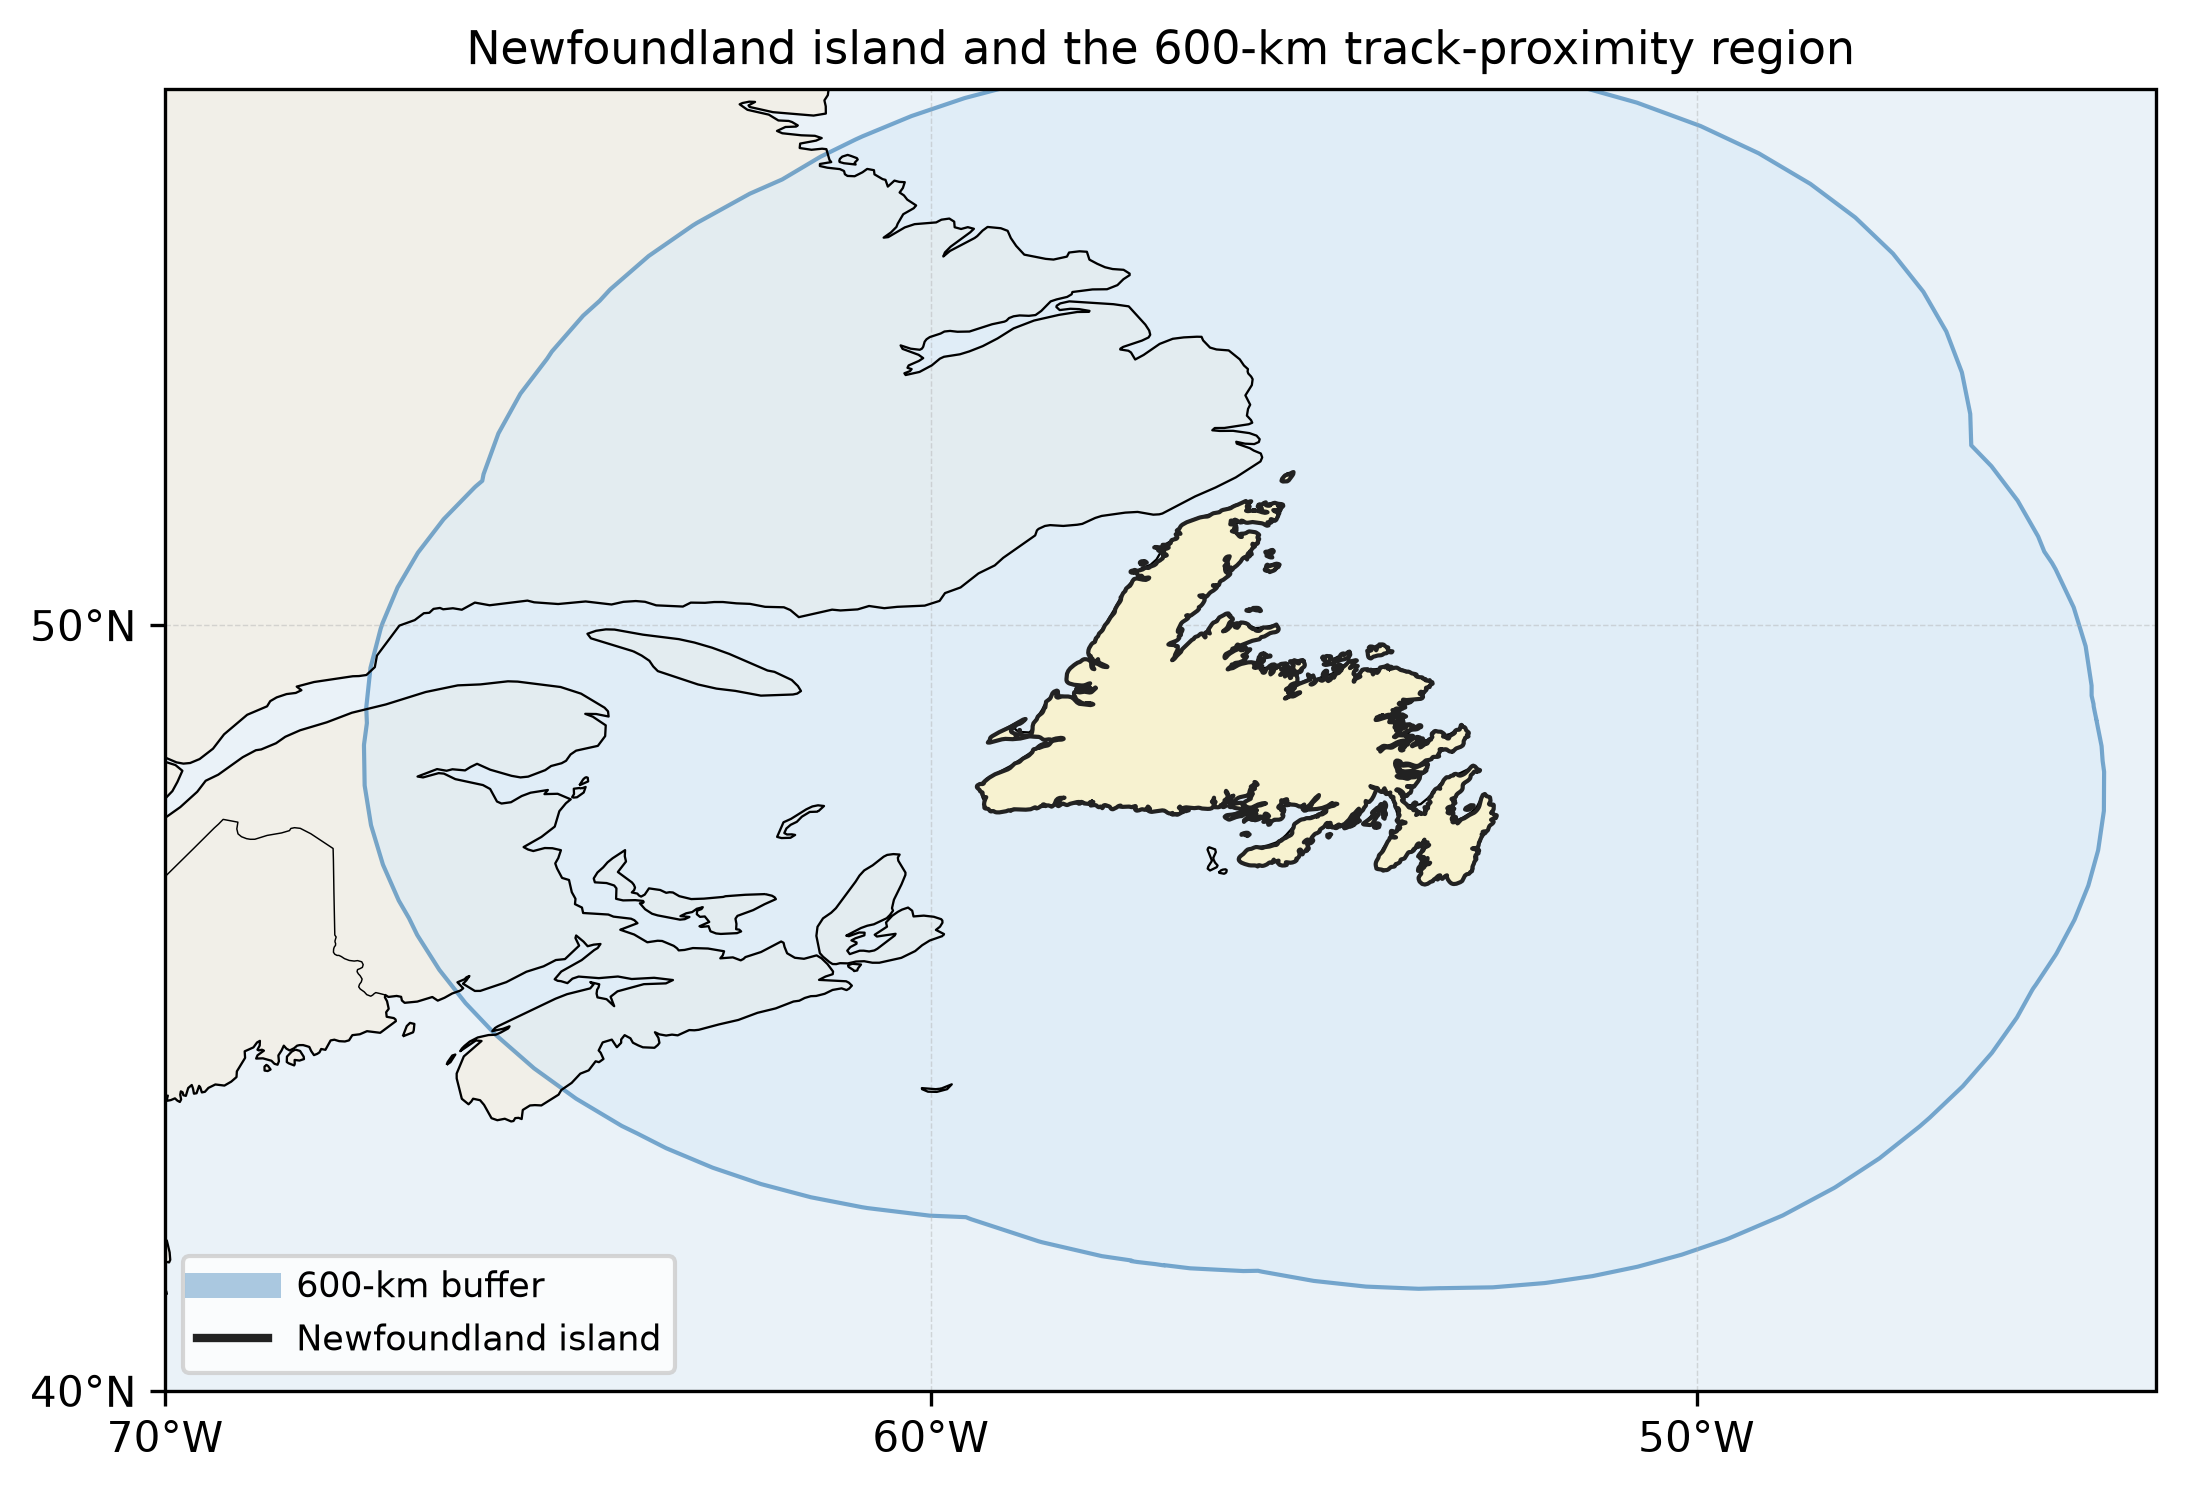
\includegraphics[width=0.78\textwidth]{figures/fig1_newfoundland_geometry.png}
\caption{Newfoundland island and its 600-km projected-distance buffer. A cyclone is classified as Newfoundland-relevant when its post-recurvature track polyline intersects this region.}
\label{fig:geometry}
\end{figure}

\subsection{Statistical analysis}
The primary estimand is the log-linear trend in annual baseline event count over 1950--2023. Annual counts were modelled using Poisson regression with a log link and centred year predictor. Effect magnitude is reported as an incidence-rate ratio (IRR) per decade with a 95\% confidence interval. Pearson \(\chi^2/\mathrm{df}\) was used to assess dispersion. As a dependence check, confidence intervals were also calculated with heteroskedasticity-and-autocorrelation-consistent covariance using two lags; Pearson-residual lag-1 correlation and a Ljung--Box test were inspected.

Two binomial models distinguish pathway behaviour from raw occurrence. The first models Newfoundland-relevant events among eligible storms. The second models Newfoundland-relevant events among detected recurvers. Both report an odds ratio (OR) per decade. Analyses were performed for 1950--2023 and for 1979--2023, with 1979 used as a fixed, coarse modern satellite-era boundary rather than an estimated changepoint. Detector and proximity sensitivities were evaluated for both periods.

Linear trends in recurvature latitude and longitude were estimated using ordinary least squares with HC3 covariance. For the joint early- versus late-era comparison, longitude and latitude were transformed to three-dimensional Earth-centred Cartesian coordinates in kilometres, and a two-sample energy-distance test was performed with 4999 permutations. Minimum-distance trends were estimated for all detected recurvers using both HC3 mean regression and median quantile regression. Results conditional on the 600-km selection were retained as secondary diagnostics. As a censoring diagnostic, both distance trends were repeated after excluding tracks whose minimum occurred at the final recorded point.

\subsection{Seasonal timing and cyclone nature}
Seasonal timing was defined by the month of the diagnosed recurvature point, not genesis or closest approach. Cyclone nature at recurvature was taken from the nearest IBTrACS source position.

\subsection{500-hPa physical-context composite}
For baseline events during 1979--2023, the 6-hourly, \(2.5^\circ\) NCEP/NCAR Reanalysis~1 500-hPa geopotential-height field was sampled at the diagnosed recurvature time \citep{Kalnay1996}. Each field was expressed as an anomaly from the corresponding 1991--2020 calendar-month mean. The \SatelliteN\ available events were composited on the native fixed North Atlantic grid and on a storm-relative \(2.5^\circ\) grid extending \(30^\circ\) west--east and \(20^\circ\) south--north from the recurvature point; storm-relative values were obtained by bilinear interpolation. Mean absolute heights are shown as contours.

At each grid point, anomaly consistency was evaluated with a two-sided one-sample \(t\)-test against zero, followed by Benjamini--Hochberg false-discovery-rate control at \(q=0.05\). The composite is illustrative and secondary: it does not remove the cyclone circulation, include a matched non-Newfoundland control, establish regional specificity or causality, or substitute for a deep-layer steering-flow analysis.

\section{Results}

\subsection{Classification and method dependence}
The baseline velocity detector identifies \AllRecurverN\ recurving storms, of which \BaselineN\ pass the 600-km Newfoundland screen. The alternative heading detector identifies \HeadingN\ relevant events and overlaps with the velocity detector for \DetectorOverlap\ storms, with Jaccard similarity \DetectorJaccard. The \DetectorDiscordantN\ discordant tracks comprise \DetectorOnlyVelocity\ velocity-only and \DetectorOnlyHeading\ heading-only classifications and are displayed in Figure~\ref{fig:discordant} for direct audit. Their disagreement demonstrates detector dependence but is not treated as an estimate of sensitivity or specificity. A separate native-cadence workflow comparison is reported in Appendix~A.

\begin{table}[htbp]
\caption{Event-list overlap between the baseline velocity and alternative heading detectors.}
\label{tab:method_comparison}
\begin{tabular}{lrrrrrl}
\toprule
Comparison & $N_1$ & $N_2$ & Both & Only 1 & Only 2 & $J$ \\
\midrule
Velocity vs. heading & 144 & 131 & 128 & 16 & 3 & 0.871 \\
\bottomrule
\end{tabular}
\end{table}


\subsection{Seasonal timing}
Baseline events occur from June through November (Figure~\ref{fig:seasonality}). \PeakMonth\ is the peak month with \PeakMonthN\ events (\PeakMonthPct\%), and August--October contains \AugOctN\ events (\AugOctPct\%). Of the \BaselineN\ events, \TropicalAtTurnN\ are coded tropical at the diagnosed turn; the remainder are subtropical, extratropical, disturbance, or uncertain classifications.

\begin{figure}[H]
\centering
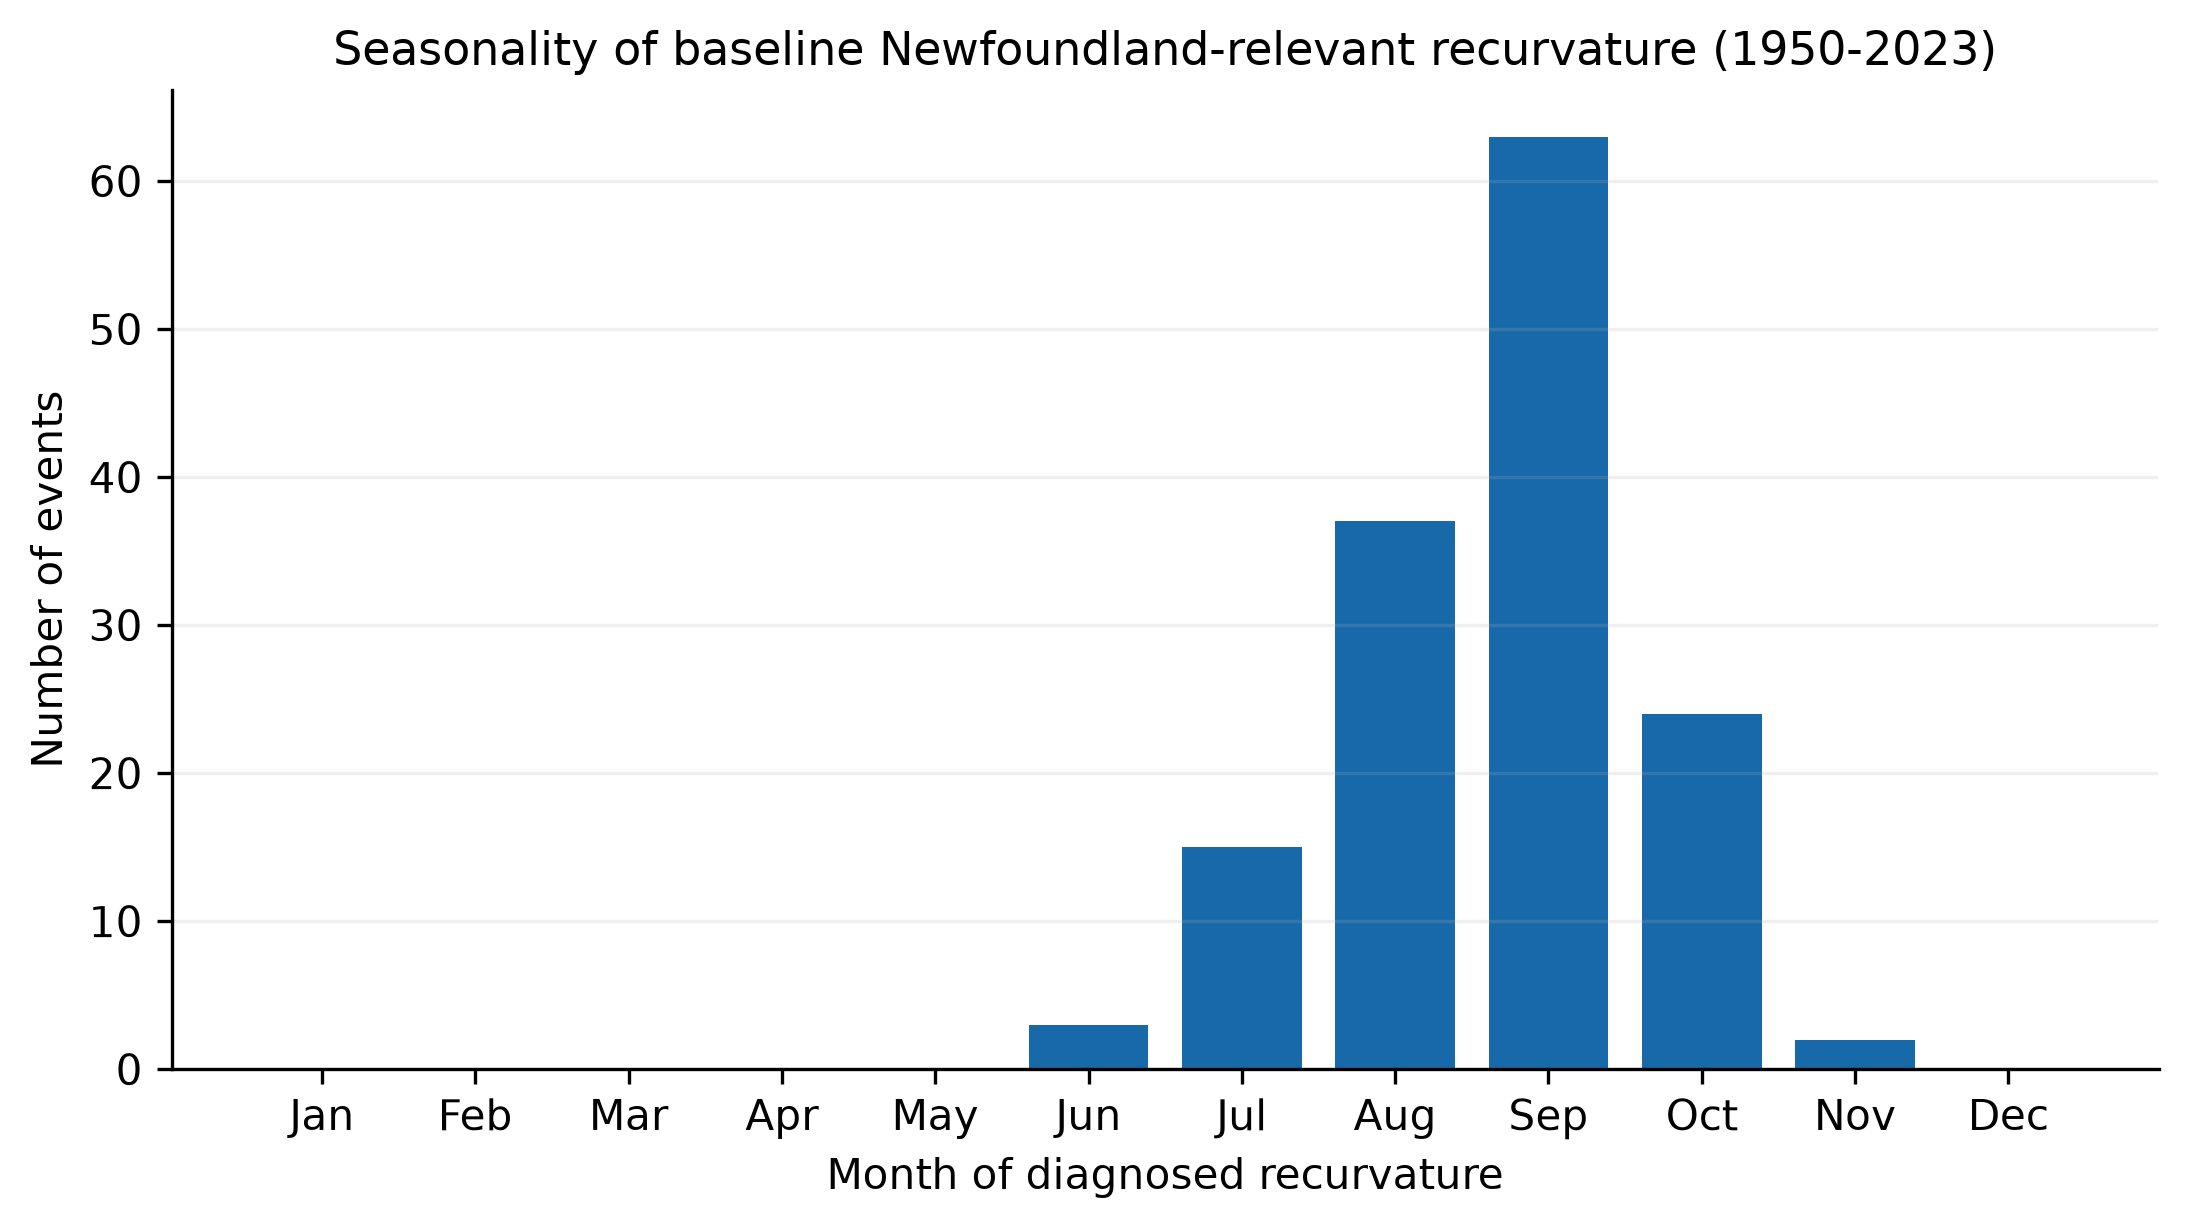
\includegraphics[width=0.82\textwidth]{figures/fig2_seasonality.png}
\caption{Month of diagnosed recurvature for the \BaselineN\ Newfoundland-relevant events identified by the baseline detector.}
\label{fig:seasonality}
\end{figure}

\subsection{Annual event frequency}
Annual counts exhibit pronounced interannual and decadal-scale variability (Figures~\ref{fig:annual}--\ref{fig:rolling}). The full-period Poisson estimate is IRR \(=\FullIRR\) per decade (95\% CI \FullCILow--\FullCIHigh; \(p=\FullP\)), with Pearson dispersion \FullDispersion. The HAC interval is \FullHACCILow--\FullHACCIHigh\ and its trend test gives \(p=\FullHACP\). Pearson-residual lag-1 autocorrelation is \FullLagOne, and the Ljung--Box test gives \(p=\FullLjungBoxP\). These diagnostics provide no indication that short-lag dependence is concealing a linear frequency trend.

For 1979--2023, the baseline model includes \SatelliteN\ events and yields IRR \(=\SatelliteIRR\) (95\% CI \SatelliteCILow--\SatelliteCIHigh; \(p=\SatelliteP\)); the HAC interval is \SatelliteHACCILow--\SatelliteHACCIHigh. The baseline point estimate therefore remains compatible with a small decrease, no change, or a substantial increase. Section~\ref{sec:sensitivity} examines its dependence on the event definition.

\begin{table}[htbp]
\caption{Poisson trend estimates for annual Newfoundland-relevant recurvature counts. HAC intervals allow for short-lag residual dependence.}
\label{tab:frequency_trends}
\begin{tabular}{lrlllll}
\toprule
Period & $N$ & IRR decade$^{-1}$ & 95\% CI & $p$ & HAC 95\% CI & Dispersion \\
\midrule
1950--2023 & 144 & 0.999 & 0.925--1.078 & 0.978 & 0.945--1.056 & 0.91 \\
1979--2023 & 86 & 1.109 & 0.942--1.307 & 0.214 & 0.980--1.256 & 1.11 \\
\bottomrule
\end{tabular}
\end{table}


\begin{figure}[H]
\centering
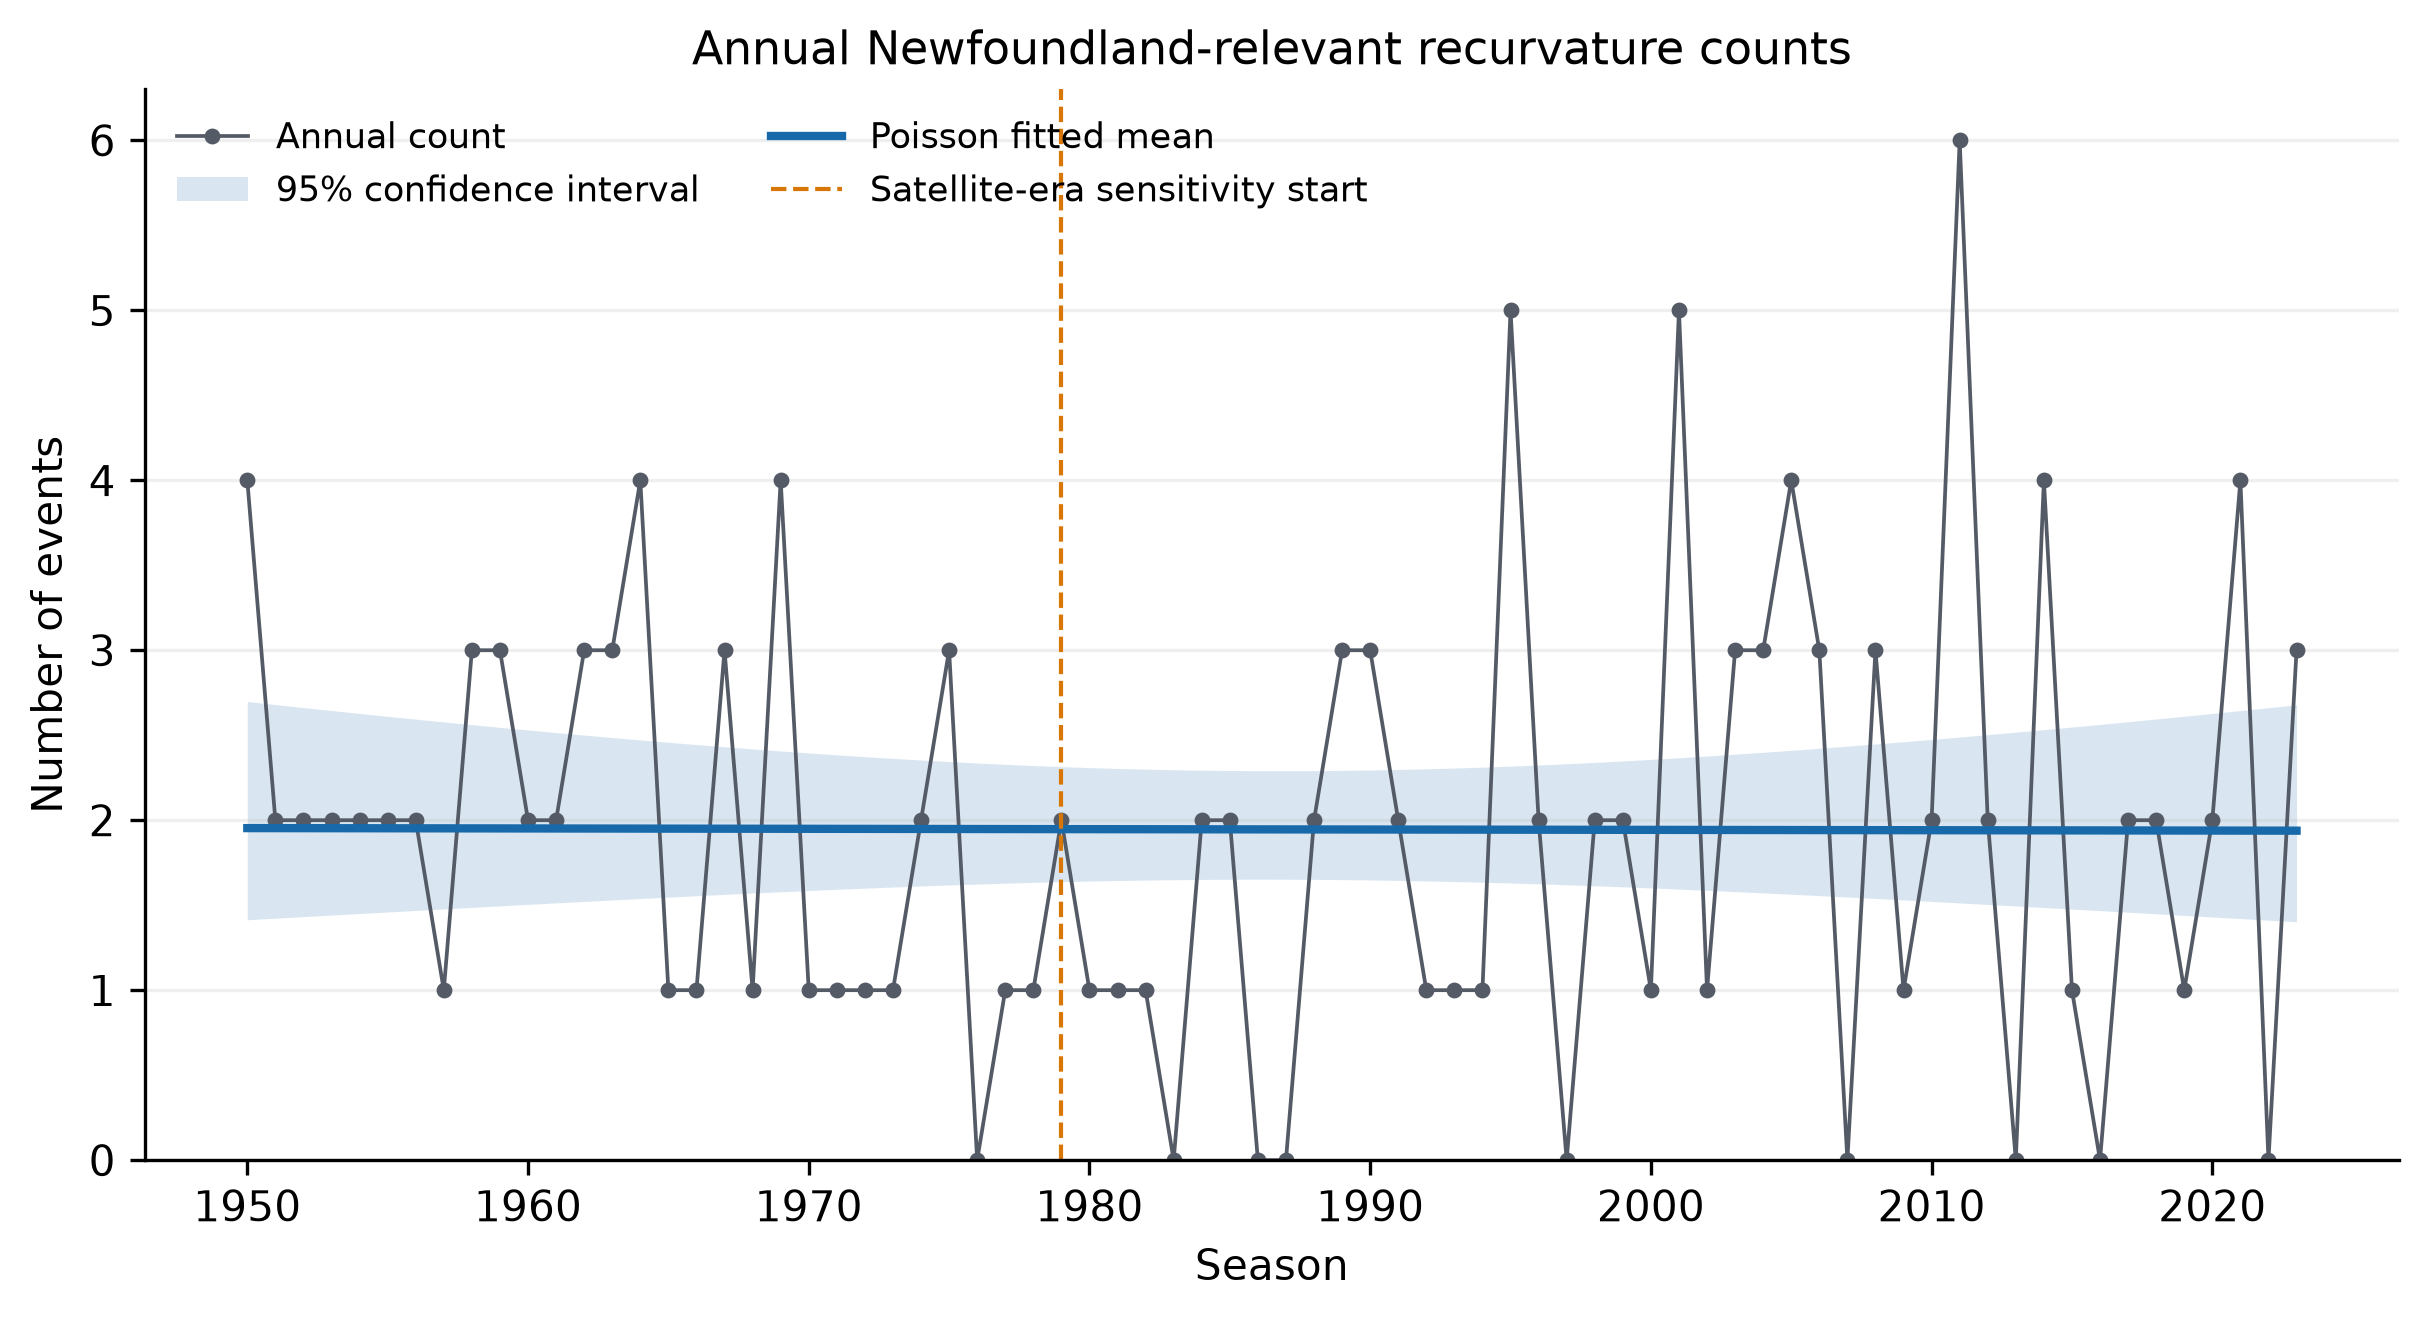
\includegraphics[width=0.94\textwidth]{figures/fig3_annual_counts_poisson.png}
\caption{Annual Newfoundland-relevant event counts from the baseline detector and the fitted Poisson mean. The shaded region is the model-based 95\% confidence interval.}
\label{fig:annual}
\end{figure}

\begin{figure}[H]
\centering
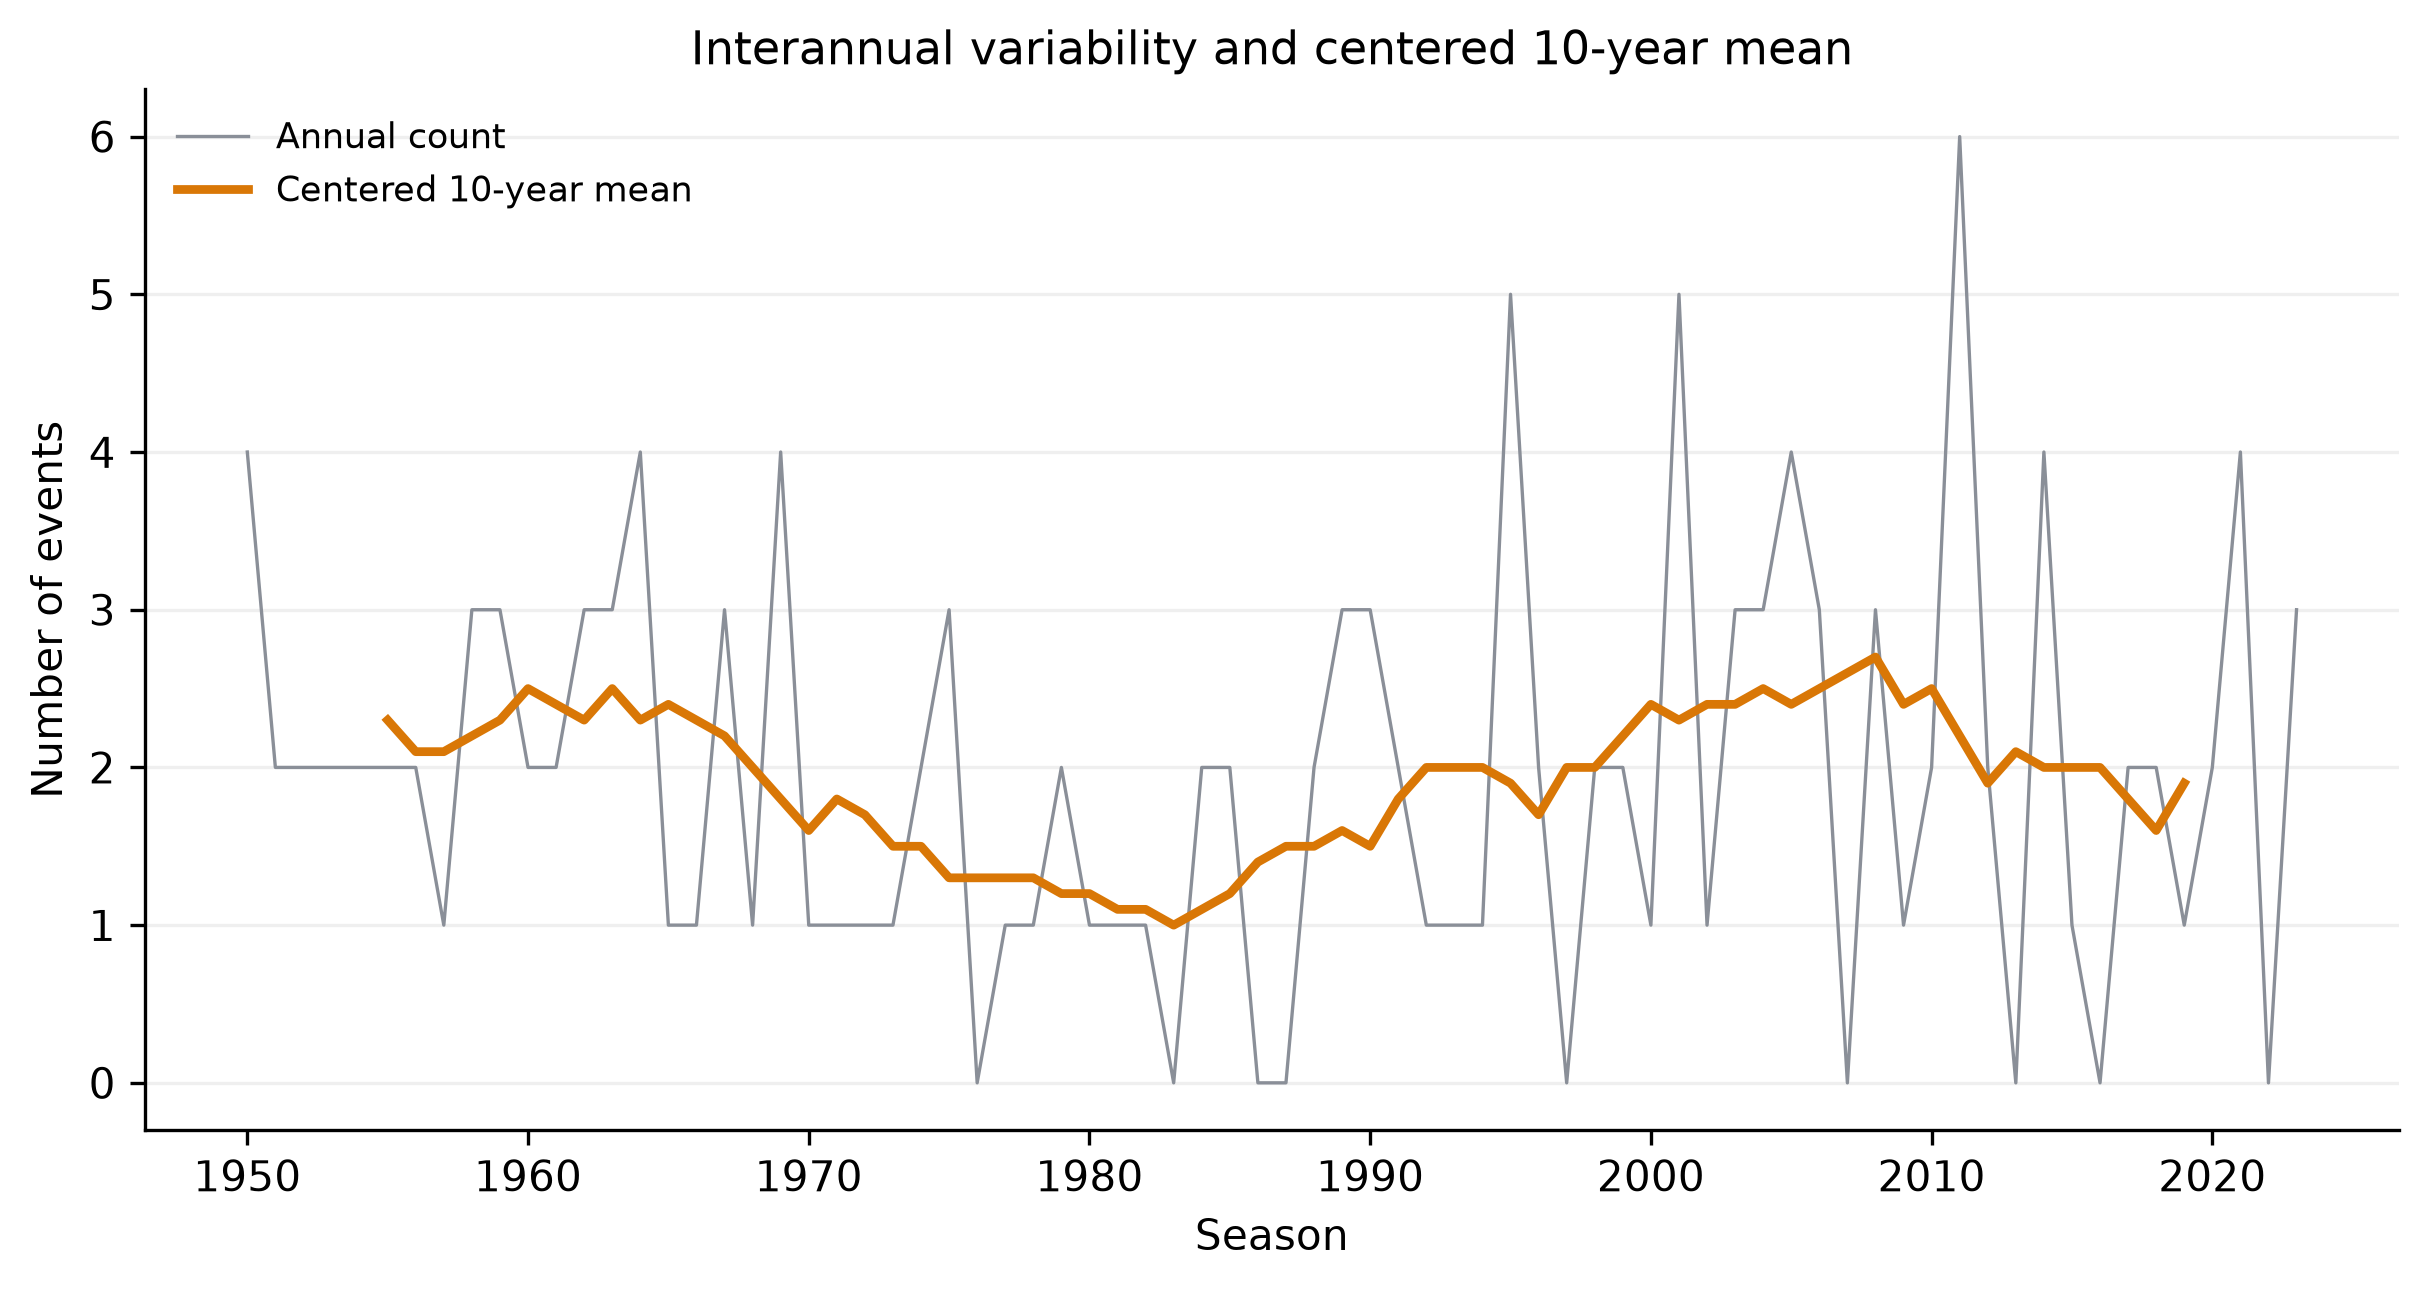
\includegraphics[width=0.94\textwidth]{figures/fig4_rolling_mean.png}
\caption{Annual event counts and a centred 10-year mean. Partial edge windows are not plotted. The smoother is descriptive and is not used for trend inference.}
\label{fig:rolling}
\end{figure}

\subsection{Pathway probabilities}
Among the \EligibleN\ eligible storms, the full-period pathway OR is \EligibleOR\ per decade (95\% CI \EligibleORLow--\EligibleORHigh; \(p=\EligibleORP\)). Among the \AllRecurverN\ detected recurvers, the corresponding OR is \RecurverOR\ (95\% CI \RecurverORLow--\RecurverORHigh; \(p=\RecurverORP\)). Satellite-era pathway estimates are also near unity (Table~\ref{tab:pathway_trends}). Thus, the positive satellite-era raw-count estimate is not accompanied by evidence that an eligible storm or recurver became increasingly likely to take a Newfoundland-relevant pathway.

\begin{table}[htbp]
\caption{Binomial trends in the probability of a Newfoundland-relevant pathway among eligible storms and among detected recurvers.}
\label{tab:pathway_trends}
\begin{tabular}{llllll}
\toprule
Denominator & Period & Events/trials & OR decade$^{-1}$ & 95\% CI & $p$ \\
\midrule
Eligible storms & 1950--2023 & 144/778 & 0.975 & 0.898--1.059 & 0.553 \\
Eligible storms & 1979--2023 & 86/470 & 1.017 & 0.853--1.213 & 0.848 \\
Detected recurvers & 1950--2023 & 144/417 & 0.940 & 0.858--1.030 & 0.185 \\
Detected recurvers & 1979--2023 & 86/263 & 0.991 & 0.812--1.209 & 0.930 \\
\bottomrule
\end{tabular}
\end{table}


\subsection{Recurvature location}
Recurvature points are broadly distributed across the western and central North Atlantic (Figure~\ref{fig:locations}). Latitude changes by \LatitudeSlope\(^{\circ}\) per decade (95\% CI \LatitudeLow--\LatitudeHigh; \(p=\LatitudeP\)), while longitude changes eastward by \LongitudeSlope\(^{\circ}\) per decade (95\% CI \LongitudeLow--\LongitudeHigh; \(p=\LongitudeP\)). The early- and late-era samples contain \EarlyN\ and \LateN\ events, respectively. Their median positions are \(\EarlyMedianLatitude^\circ\)N, \(\EarlyMedianLongitudeWest^\circ\)W and \(\LateMedianLatitude^\circ\)N, \(\LateMedianLongitudeWest^\circ\)W. The spherical-coordinate energy-distance test gives \(p=\EnergyP\), providing no evidence of an era-wide distributional displacement.

\begin{figure}[H]
\centering
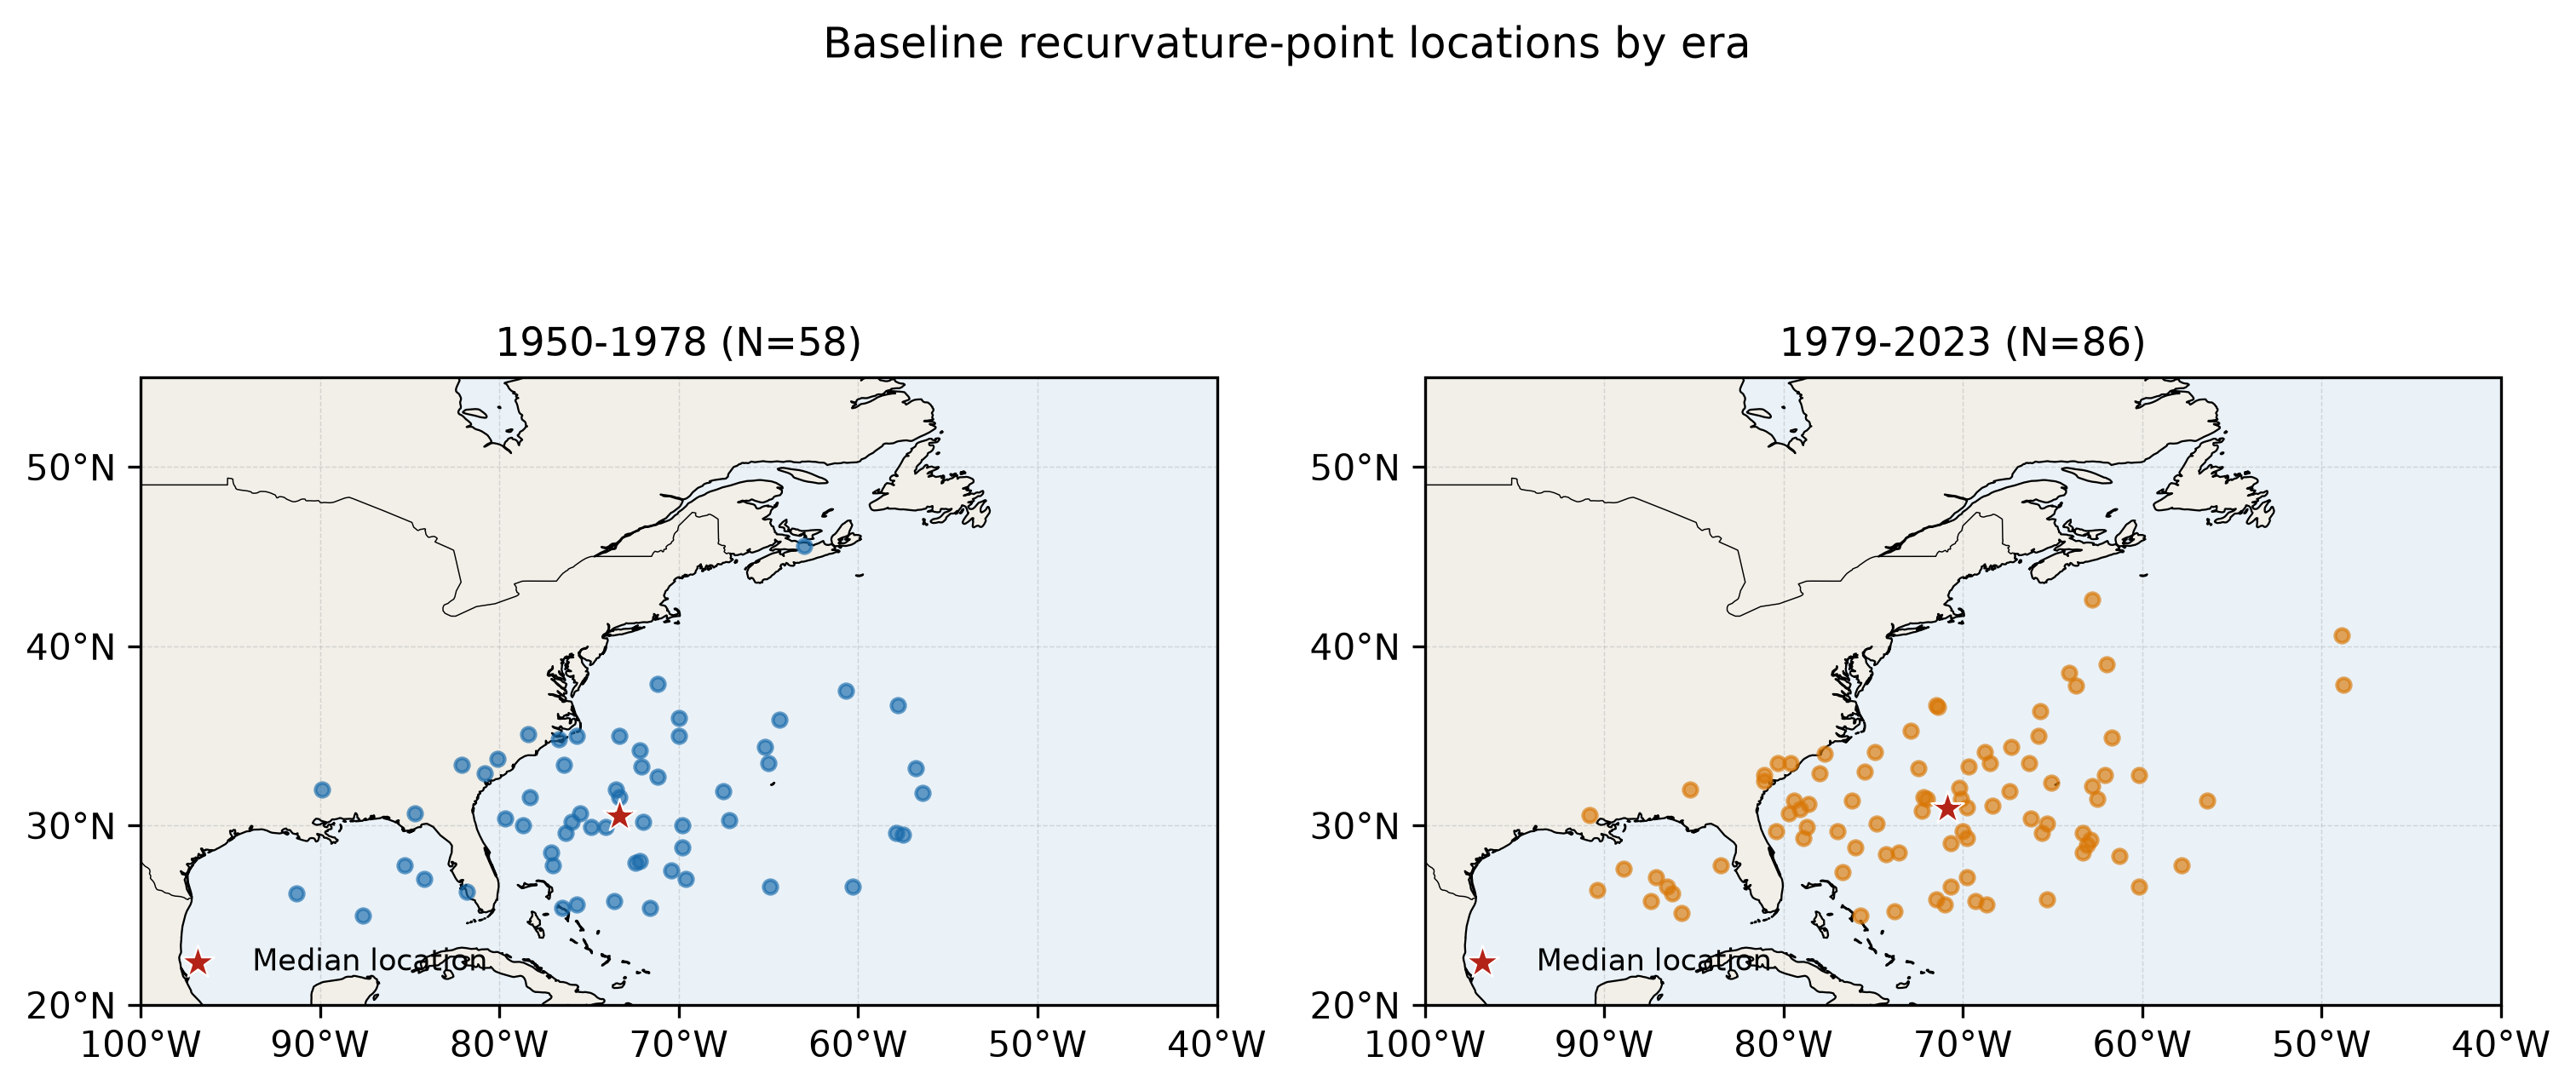
\includegraphics[width=\textwidth]{figures/fig5_recurvature_locations.png}
\caption{Recurvature-point locations for baseline Newfoundland-relevant events before and during the satellite era. Red stars identify median locations; the panels use identical domains.}
\label{fig:locations}
\end{figure}

\subsection{Post-recurvature proximity}
For all \AllRecurverN\ detected recurvers, mean minimum distance changes by \DistanceMeanSlope~km per decade (95\% CI \DistanceMeanLow--\DistanceMeanHigh; \(p=\DistanceMeanP\); Figure~\ref{fig:proximity}). Median regression yields \DistanceMedianSlope~km per decade (95\% CI \DistanceMedianLow--\DistanceMedianHigh; \(p=\DistanceMedianP\)). Median distance is \EarlyDistanceMedian~km in 1950--1978 and \LateDistanceMedian~km in 1979--2023. These estimates lean toward greater observed distance in the later period, but both intervals include no change.

\EndpointMinimumN\ of the \AllRecurverN\ tracks (\EndpointMinimumPct\%) have their minimum observed distance at the final recorded post-recurvature position, creating potential right-censoring. The corresponding proportions are similar before and during the satellite era (\EarlyEndpointPct\% and \LateEndpointPct\%). Excluding these tracks reduces the mean slope to \NonEndpointMeanSlope~km per decade (95\% CI \NonEndpointMeanLow--\NonEndpointMeanHigh; \(p=\NonEndpointMeanP\)) and the median slope to \NonEndpointMedianSlope~km per decade (95\% CI \NonEndpointMedianLow--\NonEndpointMedianHigh; \(p=\NonEndpointMedianP\); Table~\ref{tab:endpoint_sensitivity}).

When analysis is restricted to the \BaselineN\ already-selected events, the mean-distance slope reverses to \RelevantDistanceMeanSlope~km per decade (95\% CI \RelevantDistanceMeanLow--\RelevantDistanceMeanHigh; \(p=\RelevantDistanceMeanP\)). This reversal illustrates why the threshold-truncated sample is not used as the primary proximity population.

\begin{table}[htbp]
\caption{Trend estimates for recurvature-point location and minimum post-recurvature distance. Linear estimates use HC3 standard errors; the median-distance estimate uses quantile regression.}
\label{tab:location_proximity}
\begin{tabular}{lllll}
\toprule
Outcome & Sample & Effect decade$^{-1}$ & 95\% CI & $p$ \\
\midrule
Recurvature latitude & Relevant events & -0.05$^\circ$ & -0.35--0.25$^\circ$ & 0.734 \\
Recurvature longitude & Relevant events & 0.32$^\circ$ & -0.37--1.01$^\circ$ & 0.364 \\
Mean minimum distance & All recurvers & 25.9 km & -10.1--61.9 km & 0.158 \\
Median minimum distance & All recurvers & 38.1 km & -11.0--87.2 km & 0.129 \\
\bottomrule
\end{tabular}
\end{table}

\begin{table}[htbp]
\caption{Sensitivity of minimum-distance trends to post-recurvature tracks whose closest observed location is the final recorded point. Slopes are in km decade$^{-1}$.}
\label{tab:endpoint_sensitivity}
\resizebox{\textwidth}{!}{%
\begin{tabular}{lrllll}
\toprule
Sample & $N$ & Mean slope (95\% CI) & Mean $p$ & Median slope (95\% CI) & Median $p$ \\
\midrule
All detected recurvers & 417 & 25.9 (-10.1--61.9) & 0.158 & 38.1 (-11.0--87.2) & 0.129 \\
Excluding endpoint minima & 249 & 16.9 (-20.6--54.5) & 0.376 & 14.7 (-39.0--68.4) & 0.592 \\
\bottomrule
\end{tabular}%
}
\end{table}


\begin{figure}[H]
\centering
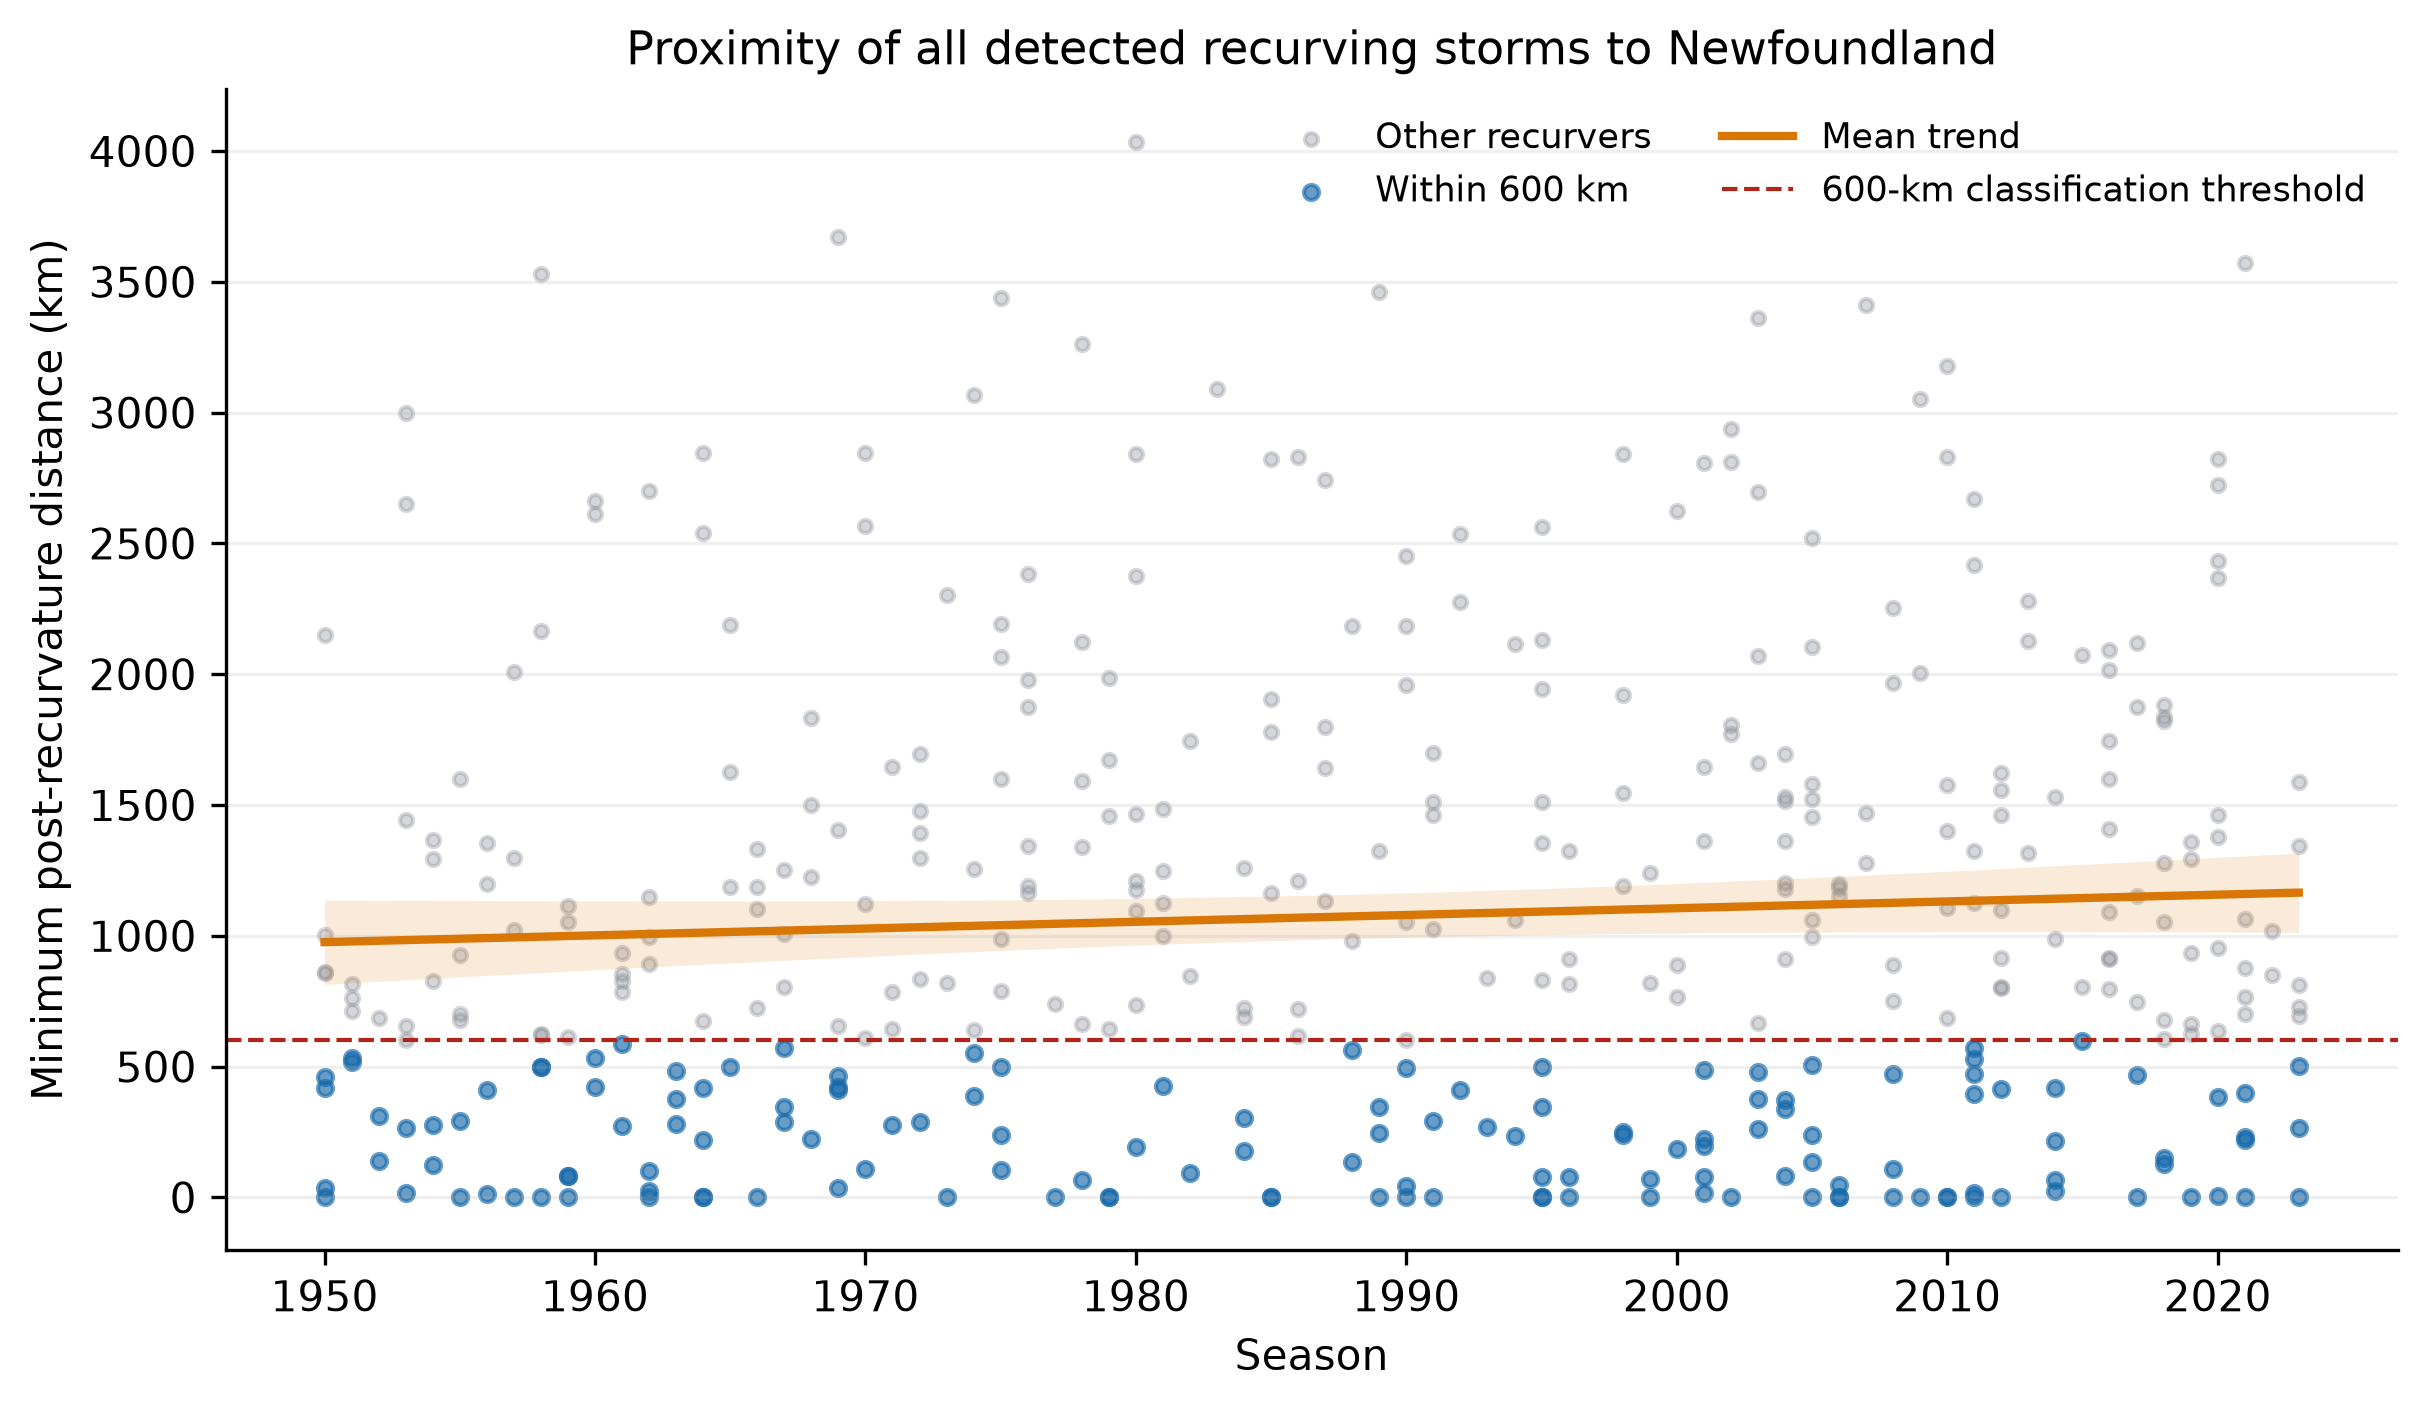
\includegraphics[width=0.95\textwidth]{figures/fig6_proximity_all_recurvers.png}
\caption{Minimum post-recurvature distance to Newfoundland for every recurver identified by the baseline detector. Blue points satisfy the 600-km classification; grey points retain the untruncated proximity distribution.}
\label{fig:proximity}
\end{figure}

\begin{figure}[H]
\centering
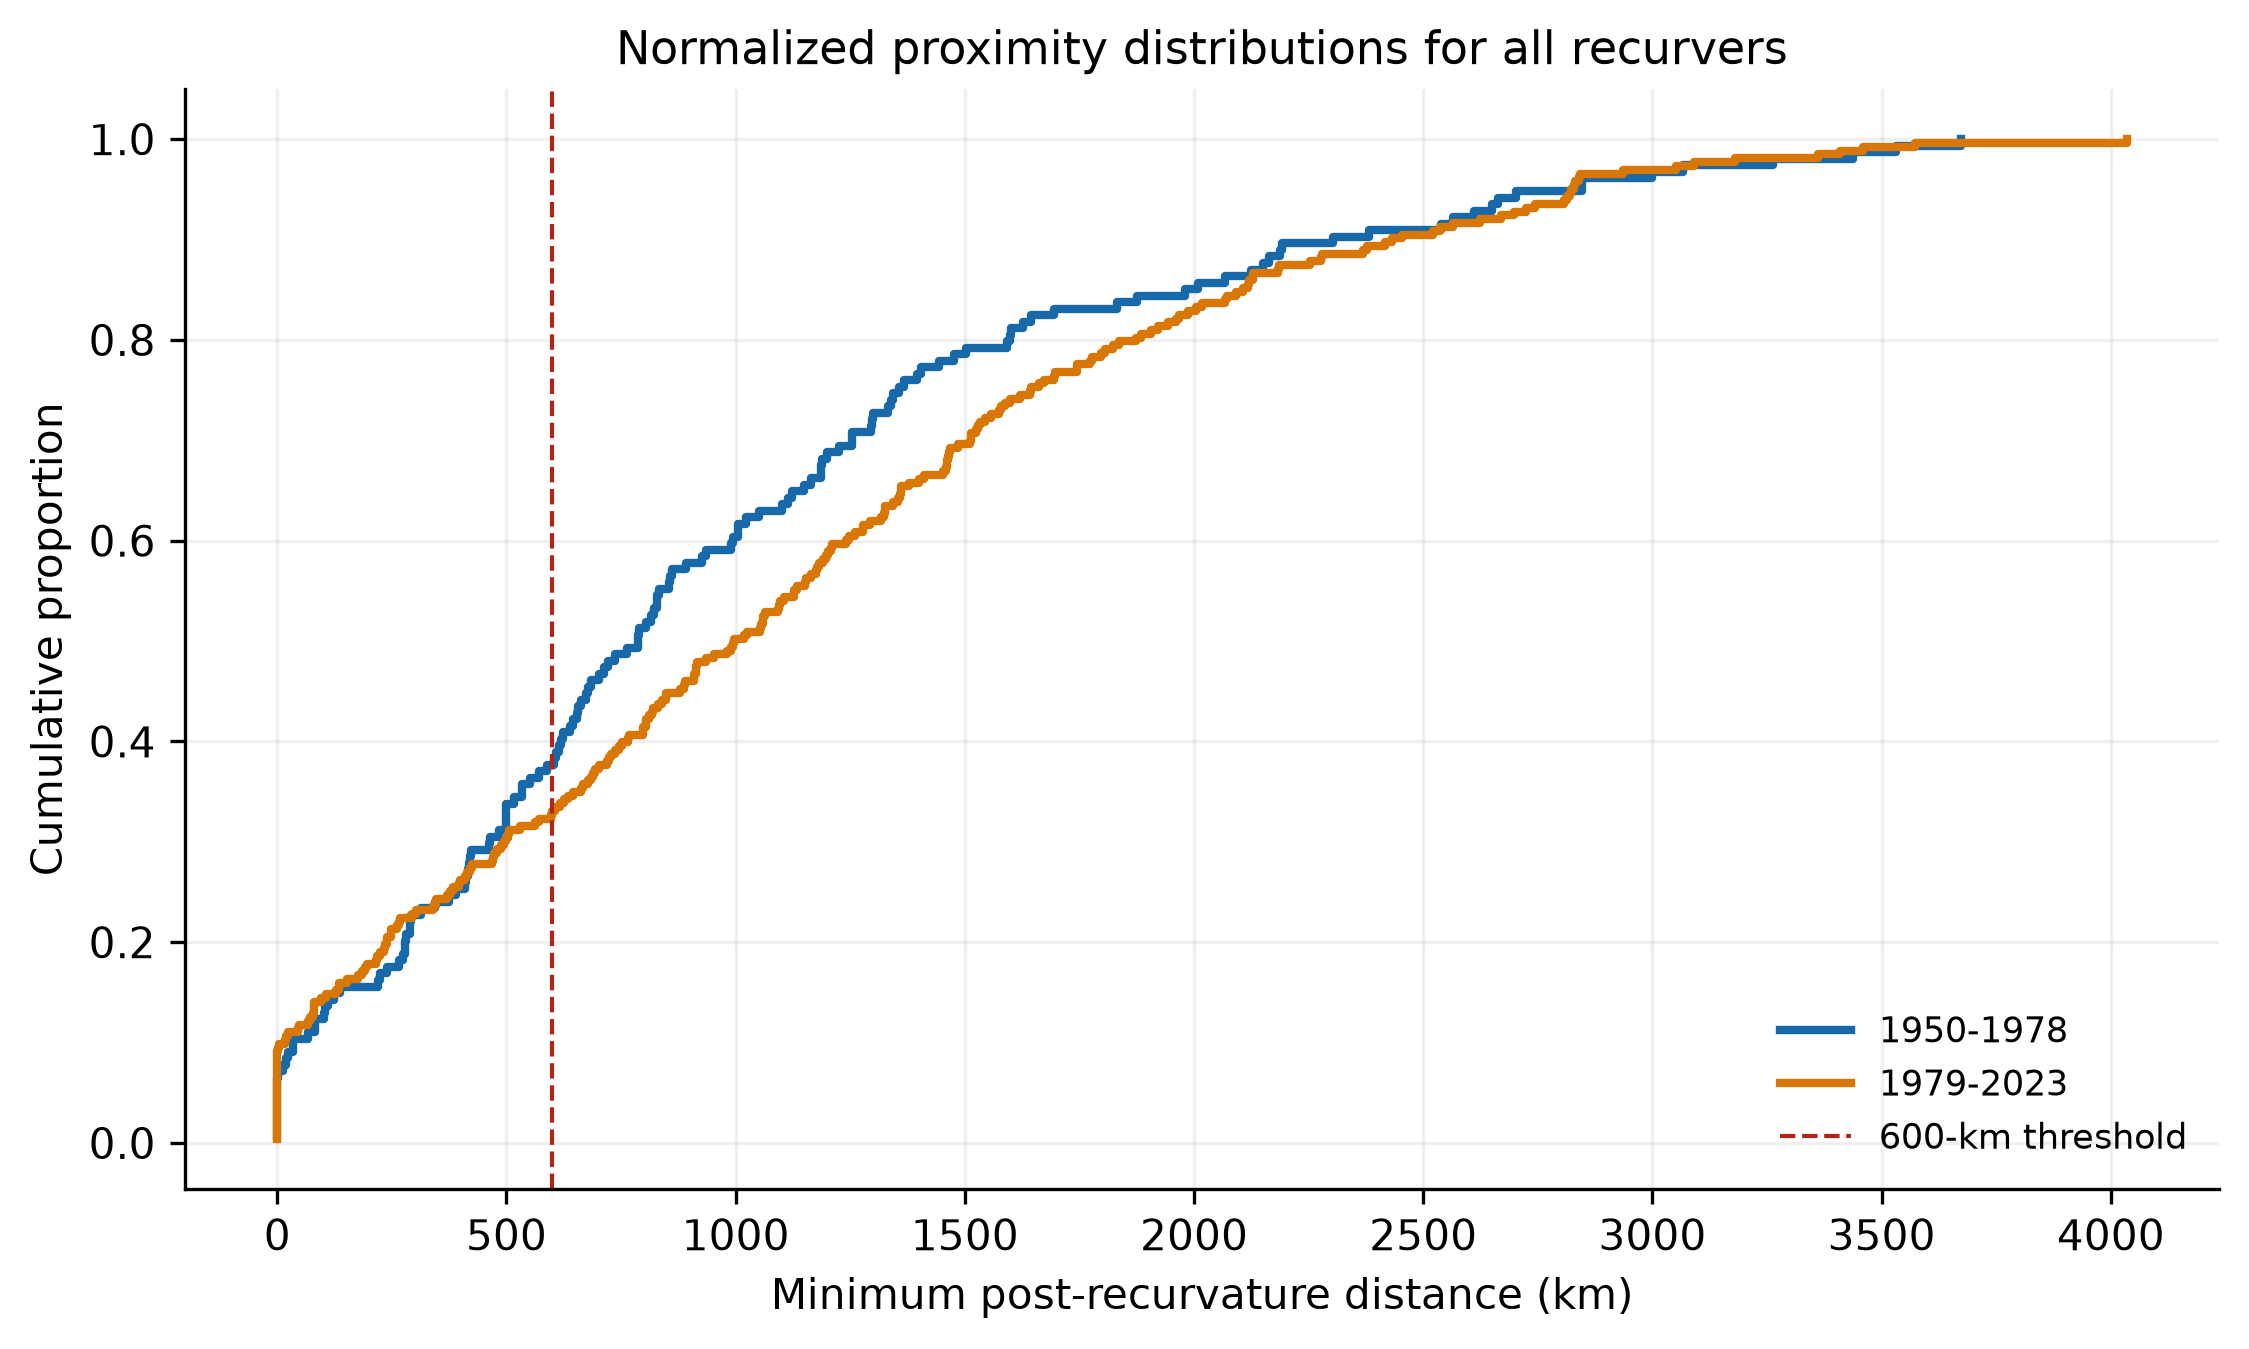
\includegraphics[width=0.88\textwidth]{figures/fig7_proximity_ecdf.png}
\caption{Empirical cumulative distributions of minimum distance for all recurvers by era. Curves are normalized within each era, avoiding the unequal-sample-size distortion of raw-frequency histograms.}
\label{fig:proximity_ecdf}
\end{figure}

\subsection{Sensitivity to proximity and detector settings}
\label{sec:sensitivity}
The exact event count depends materially on the proximity threshold: it increases from \ThresholdLowN\ at 300~km to \ThresholdHighN\ at 1000~km (Table~\ref{tab:threshold_sensitivity}; Figure~\ref{fig:threshold}). The full-period trend estimate is much less sensitive: IRRs span \ThresholdFullIRRMin--\ThresholdFullIRRMax\ across these thresholds, and every interval includes unity.

Across the 24 detector configurations, the full-period event count ranges from \DetectorEventMin\ to \DetectorEventMax\ and the IRR ranges from \DetectorFullIRRMin\ to \DetectorFullIRRMax. No full-period configuration produces a statistically resolved monotonic trend. Consequently, the full-period qualitative interpretation is stable, but \BaselineN\ should not be treated as a definition-free estimate of the number of historically relevant storms.

The satellite-era raw-count result is less stable. Across proximity thresholds, IRRs range from \ThresholdSatelliteIRRMin\ to \ThresholdSatelliteIRRMax; at 1000~km, \ThresholdHighSatelliteN\ events yield IRR \(=\ThresholdHighSatelliteIRR\) (95\% CI \ThresholdHighSatelliteLow--\ThresholdHighSatelliteHigh; \(p=\ThresholdHighSatelliteP\); Table~\ref{tab:satellite_threshold_sensitivity}). Across detector configurations, satellite-era IRRs range from \DetectorSatelliteIRRMin\ to \DetectorSatelliteIRRMax. One model-based interval excludes unity: the \(25^\circ\)N, \DetectorSensitiveWindow-hour, \DetectorSensitiveThreshold~km~h\(^{-1}\) configuration yields \(N=\DetectorSensitiveSatelliteN\), IRR \(=\DetectorSensitiveSatelliteIRR\) (95\% CI \DetectorSensitiveSatelliteLow--\DetectorSensitiveSatelliteHigh; \(p=\DetectorSensitiveSatelliteP\)); six HAC intervals exclude unity. In contrast, none of the corresponding conditional pathway models among eligible storms or detected recurvers resolves a trend. Thus, evidence for a satellite-era increase in raw event opportunity is definition-sensitive, while evidence for an increasing conditional Newfoundland pathway is absent across the tested grid.

The alternative Newfoundland-centred azimuthal-equidistant projection classifies \ProjectionAlternativeN\ events, changing \ProjectionClassificationChanges\ boundary cases relative to EPSG:3347. Basin-wide distances correlate at \(r=\ProjectionDistanceCorrelation\), with a median absolute difference of \ProjectionMedianAbsoluteDifference~km. The alternative-projection mean-distance trend is \ProjectionAlternativeMeanSlope~km per decade (95\% CI \ProjectionAlternativeMeanLow--\ProjectionAlternativeMeanHigh; \(p=\ProjectionAlternativeMeanP\)), leaving the interpretation unchanged.

\begin{table}[htbp]
\caption{Sensitivity of event classification and Poisson trend estimates to the Newfoundland-island proximity threshold.}
\label{tab:threshold_sensitivity}
\begin{tabular}{rrlllll}
\toprule
Threshold (km) & $N$ & IRR decade$^{-1}$ & CI low & CI high & $p$ & Dispersion \\
\midrule
300 & 95 & 1.023 & 0.931 & 1.124 & 0.640 & 0.739 \\
500 & 132 & 1.002 & 0.925 & 1.086 & 0.955 & 0.922 \\
600 & 144 & 0.999 & 0.925 & 1.078 & 0.978 & 0.913 \\
800 & 188 & 0.994 & 0.929 & 1.062 & 0.851 & 0.957 \\
1000 & 225 & 1.003 & 0.944 & 1.067 & 0.912 & 1.017 \\
\bottomrule
\end{tabular}
\end{table}

\begin{table}[htbp]
\caption{Satellite-era sensitivity to the Newfoundland-island proximity threshold. Conditional odds ratios use the eligible-storm and detected-recurver denominators.}
\label{tab:satellite_threshold_sensitivity}
\resizebox{\textwidth}{!}{%
\begin{tabular}{rrllll}
\toprule
Threshold (km) & $N$ & Count IRR (95\% CI) & $p$ & Eligible-storm OR (95\% CI) & Recurver OR (95\% CI) \\
\midrule
300 & 60 & 1.070 (0.880--1.300) & 0.499 & 0.977 (0.797--1.197) & 0.947 (0.758--1.182) \\
500 & 80 & 1.079 (0.911--1.279) & 0.376 & 0.986 (0.823--1.181) & 0.953 (0.779--1.168) \\
600 & 86 & 1.109 (0.942--1.307) & 0.214 & 1.017 (0.853--1.213) & 0.991 (0.812--1.209) \\
800 & 109 & 1.156 (0.999--1.337) & 0.052 & 1.071 (0.911--1.260) & 1.061 (0.877--1.283) \\
1000 & 132 & 1.187 (1.039--1.356) & 0.012 & 1.115 (0.957--1.299) & 1.130 (0.937--1.364) \\
\bottomrule
\end{tabular}%
}
\end{table}


\begin{figure}[H]
\centering
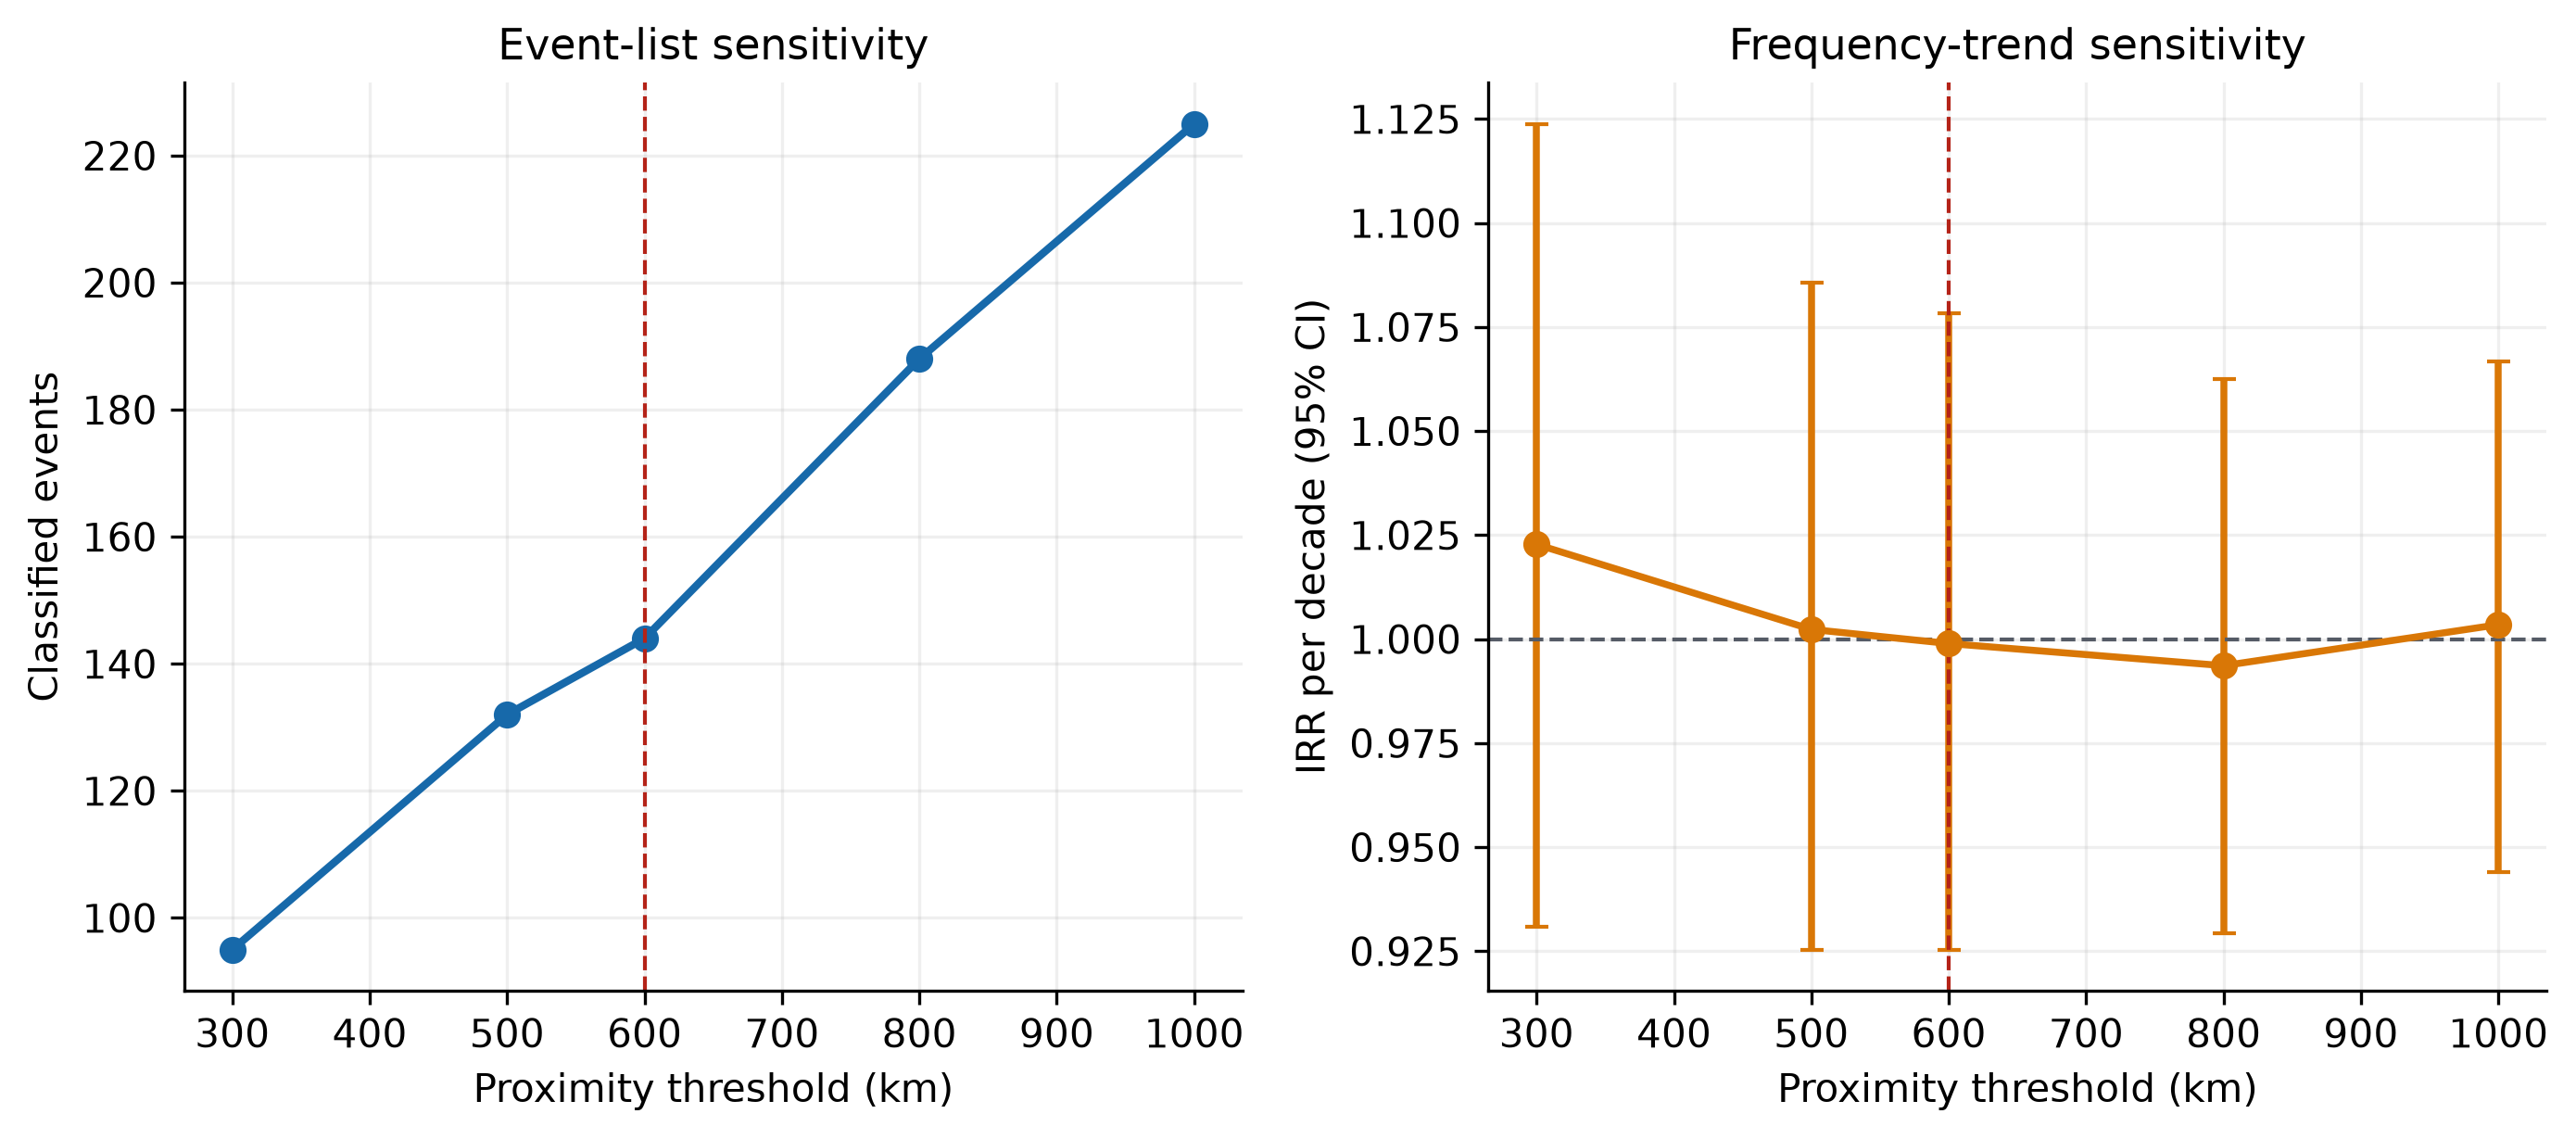
\includegraphics[width=0.94\textwidth]{figures/fig8_threshold_sensitivity.png}
\caption{Full-period sensitivity of event-list size (left) and the Poisson frequency trend (right) to the track-proximity threshold. The 600-km baseline is marked in red.}
\label{fig:threshold}
\end{figure}

\subsection{Illustrative 500-hPa physical context}
The geographic composite contains a positive height anomaly centred near Newfoundland and Atlantic Canada, accompanied by negative anomalies farther east (Figure~\ref{fig:composite}a). Because recurvature points span a broad region, the storm-relative panel provides the clearer dynamical geometry: a positive anomaly is centred approximately \(10^\circ\)--\(20^\circ\) northeast of the recurvature point, while lower anomalous heights occur near and slightly west of the cyclone (Figure~\ref{fig:composite}b). The absolute-height contours and anomaly pattern are consistent with a common downstream ridge signal during the diagnosed turn.

The negative anomaly near the storm may include the cyclone circulation itself. Without a matched non-Newfoundland recurver composite, neither panel establishes that the pattern is regionally specific or proves a single steering mechanism. The composite should therefore be interpreted only as environmental context rather than attribution.

\begin{figure}[H]
\centering
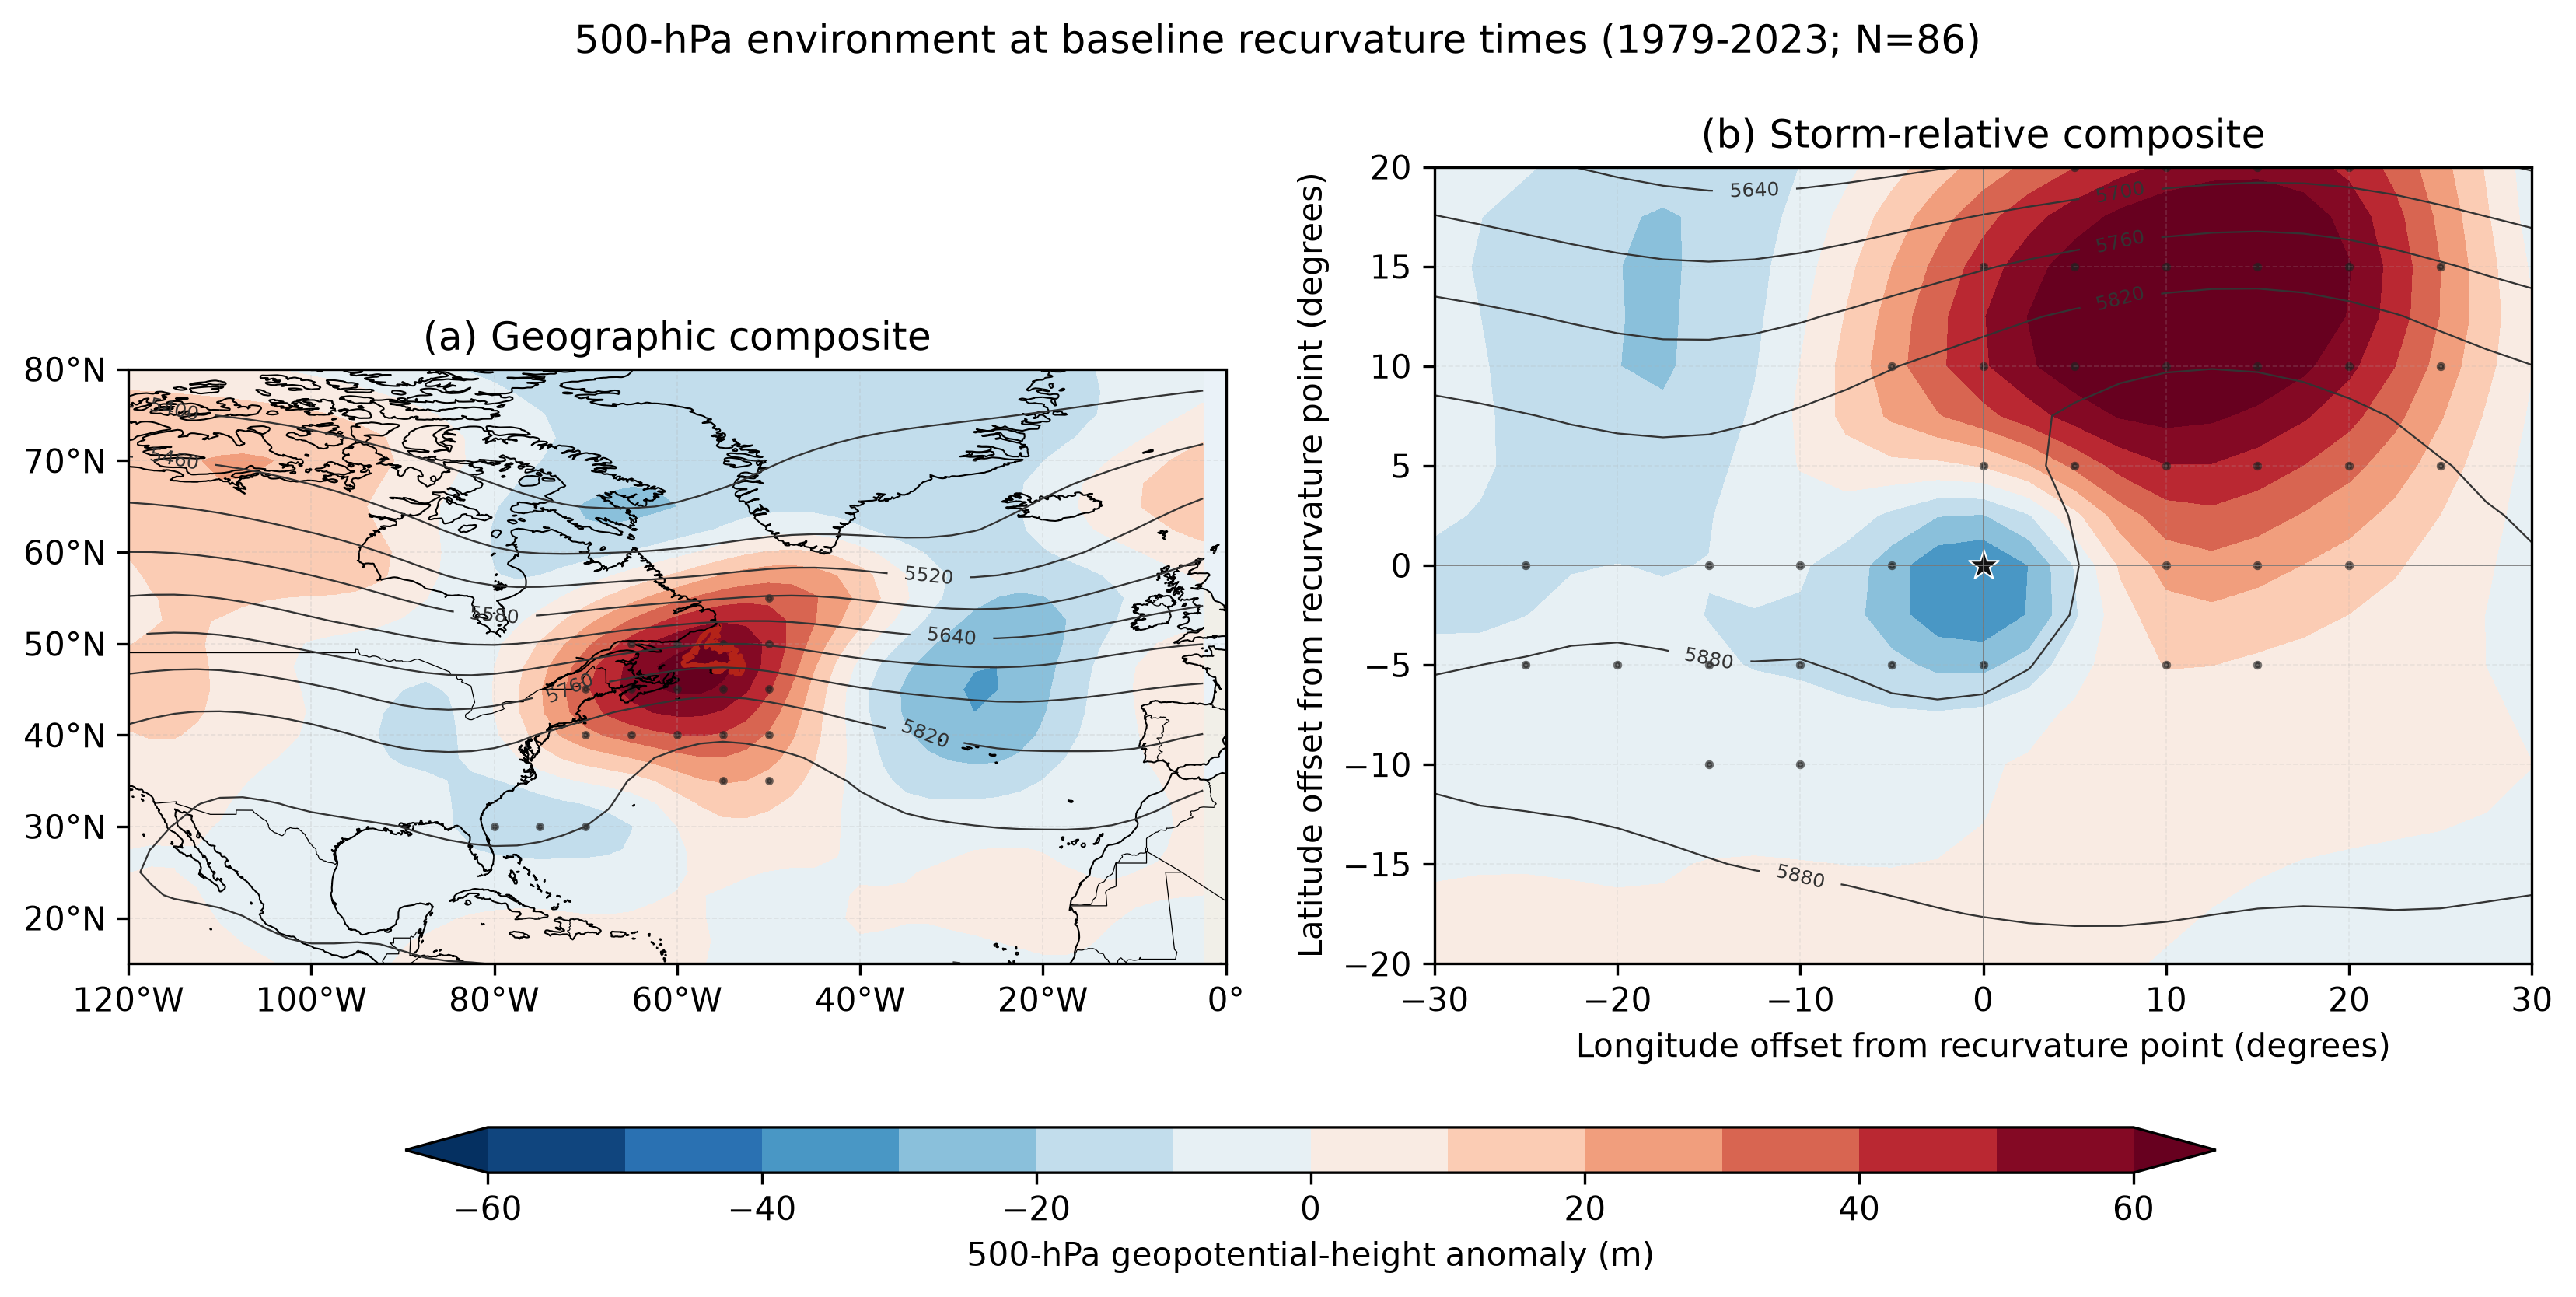
\includegraphics[width=\textwidth]{figures/fig9_z500_composite.png}
\caption{Mean 500-hPa geopotential-height anomaly at satellite-era recurvature times identified by the baseline detector. Panel (a) is composited on a fixed geographic grid; Newfoundland is outlined in red. Panel (b) is composited relative to each recurvature point, marked by the star. Black contours show mean absolute height in metres. Stippling denotes grid points passing a two-sided test against zero after false-discovery-rate control at \(q=0.05\).}
\label{fig:composite}
\end{figure}

\section{Discussion}

\subsection{Principal interpretation}
The uniform-grid analysis finds no detectable monotonic change in the annual count of Newfoundland-relevant recurvature events during 1950--2023 under the baseline definition. This conclusion is supported by standard and autocorrelation-robust intervals, proximity-threshold tests, a physically constrained detector grid, and projection sensitivity. It does not demonstrate that the physical climate system is unchanged. Under the fitted constant log-linear model, the full-period per-decade confidence interval corresponds to an endpoint rate ratio of approximately \FullRecordFactorLow--\FullRecordFactorHigh\ across 1950--2023. The study therefore does not establish equivalence or rule out climatically meaningful changes that are too small or variable to resolve with this sample.

The same variability-dominated interpretation applies to pathway probability and recurvature location. The location results are no longer based solely on visual overlap: separate latitude and longitude estimates and a joint spatial test all remain non-robust.

\subsection{Satellite-era behaviour}
The baseline 1979--2023 raw-count point estimate corresponds to an approximately 11\% increase per decade, but its uncertainty is broad; its confidence interval corresponds to an endpoint rate ratio of approximately \SatelliteRecordFactorLow--\SatelliteRecordFactorHigh\ across the satellite-era analysis period. Some broader proximity thresholds and shorter-window detector settings resolve a positive raw-count trend, whereas the baseline and most alternatives do not. The defensible interpretation is therefore not that the satellite-era increase is uniformly absent, but that its statistical resolution depends on how a Newfoundland-relevant event is defined.

Neither satellite-era pathway-probability model shows a comparable increase, and no conditional pathway model resolves a trend across the tested threshold and detector grids. Changes in basin-wide storm opportunity could therefore contribute to the raw-count signal without a systematic change in the conditional pathway toward Newfoundland. Sampling variability remains another sufficient explanation.

\subsection{Proximity}
The all-recurver proximity estimates point toward greater observed distance in later years, but neither interval excludes no change. More importantly, approximately two-fifths of all recurvers attain their minimum distance at the final recorded track position. Although the proportion is nearly identical across eras and post-recurvature track duration has no detectable trend, excluding these potentially right-censored cases substantially attenuates the median estimate. The proximity result should therefore be treated as exploratory rather than near-significant evidence of a physical displacement. The opposite-signed estimate within the 600-km subset is a selection effect rather than evidence of contradictory physical changes.

\subsection{Classification uncertainty}
Temporal standardization gives each detector window a fixed physical duration, but it does not make recurvature unique. Event counts vary substantially with latitude gate, window length, eastward-speed threshold, and regional distance threshold. The alternative heading detector agrees on most events, but neither detector has been tested against an independent expert-labelled recurvature archive. The defensible claim is therefore robustness of the full-period near-unity trend estimate across operational definitions, not validated detector skill or certainty that precisely \BaselineN\ storms form the only valid historical list.

\subsection{Regional interpretation and limitations}
The September maximum and concentration during August--October are directly useful for seasonal monitoring. The 600-km classification should not, however, be presented as an impact record. A weak cyclone at 400~km and a large transitioning cyclone at the same distance have different hazard footprints. Intensity, size, frontal evolution, waves, rainfall, and observed Newfoundland impacts are outside the current analysis.

Earlier best-track data are less homogeneous than the satellite-era record \citep{LandseaFranklin2013}. Linear interpolation cannot recover unobserved track detail, Natural Earth geometry introduces finite coastline resolution, and projected distances are not identical across coordinate systems. The projection sensitivity indicates that these geometric choices affect a few boundary classifications but not the trend interpretation. The 500-hPa composite includes the cyclone circulation, only one pressure level, and no matched control population; it cannot establish Newfoundland-specific dynamics. Finally, linear models summarize monotonic change but do not fully describe decadal clustering or nonlinear variability.

\subsection{Future work}
Future work should connect track proximity to intensity, storm size, extratropical-transition phase, and verified Newfoundland impacts. Deep-layer steering-flow and potential-vorticity composites should be compared with matched non-Newfoundland recurvers. Track uncertainty could be propagated through the detector using perturbed-track ensembles. A separate coastline-intersection analysis would also distinguish landfalls from offshore hazard pathways without conflating the two.

\section{Conclusions}
After placing IBTrACS tracks on a regular 6-hour grid and requiring a sustained west-to-east, poleward transition, \BaselineN\ North Atlantic cyclones of tropical origin are classified within 600~km of Newfoundland after recurvature during 1950--2023.

The full-period annual count shows essentially no monotonic trend (IRR \(=\FullIRR\) per decade, 95\% CI \FullCILow--\FullCIHigh). Conditional pathway probabilities and recurvature-point location also show no robust change. Satellite-era annual counts have a positive signal whose statistical resolution varies with detector and distance definition, without a corresponding increase in conditional pathway probability. Minimum observed distance among all recurvers may have increased, but the estimate is non-robust and sensitive to potential end-of-track censoring. September is the dominant recurvature month, and \AugOctPct\% of events occur during August--October.

Sensitivity experiments separate two conclusions that should not be confused: the near-unity full-period trend is stable across reasonable definitions, while the exact event count is not. Newfoundland-relevant recurvature is therefore best described as a variable pathway climatology with no resolved monotonic frequency or location trend under the baseline definitions.

\section*{Appendix A: Native-cadence workflow comparison}
A diagnostic comparator was applied directly to the native-cadence source positions to quantify the combined influence of temporal processing, trajectory criteria, eligibility, and regional screening. It required at least 25 valid source positions and identified the first point at or north of \(25^\circ\)N for which mean zonal displacement over four source increments changed from at most 30~km per increment to more than 30~km per increment. Regional relevance was then assigned when the post-detection track entered a Newfoundland-centred latitude--longitude envelope or passed within 600~km of one of five representative points.

Applied to the same tropical-origin source population, this comparator identifies \LegacyN\ events. Of these, \LegacyOverlap\ overlap with the \BaselineN\ baseline events; \LegacyOnly\ occur only in the native-cadence list and \BaselineOnlyLegacyComparison\ only in the baseline list, giving Jaccard similarity \LegacyJaccard. Because source increments vary in duration and the comparator also differs in trajectory and regional criteria, this is a workflow-level comparison rather than a sensitivity test of one isolated parameter. It is not used for the primary frequency, location, or proximity inference.

\section*{Appendix B: Detector-discordant events}
Figure~\ref{fig:discordant} provides a transparent visual audit of all detector-discordant relevant events. It is not a blinded validation set, and no accuracy statistic is inferred from it.
\begin{figure}[H]
\centering
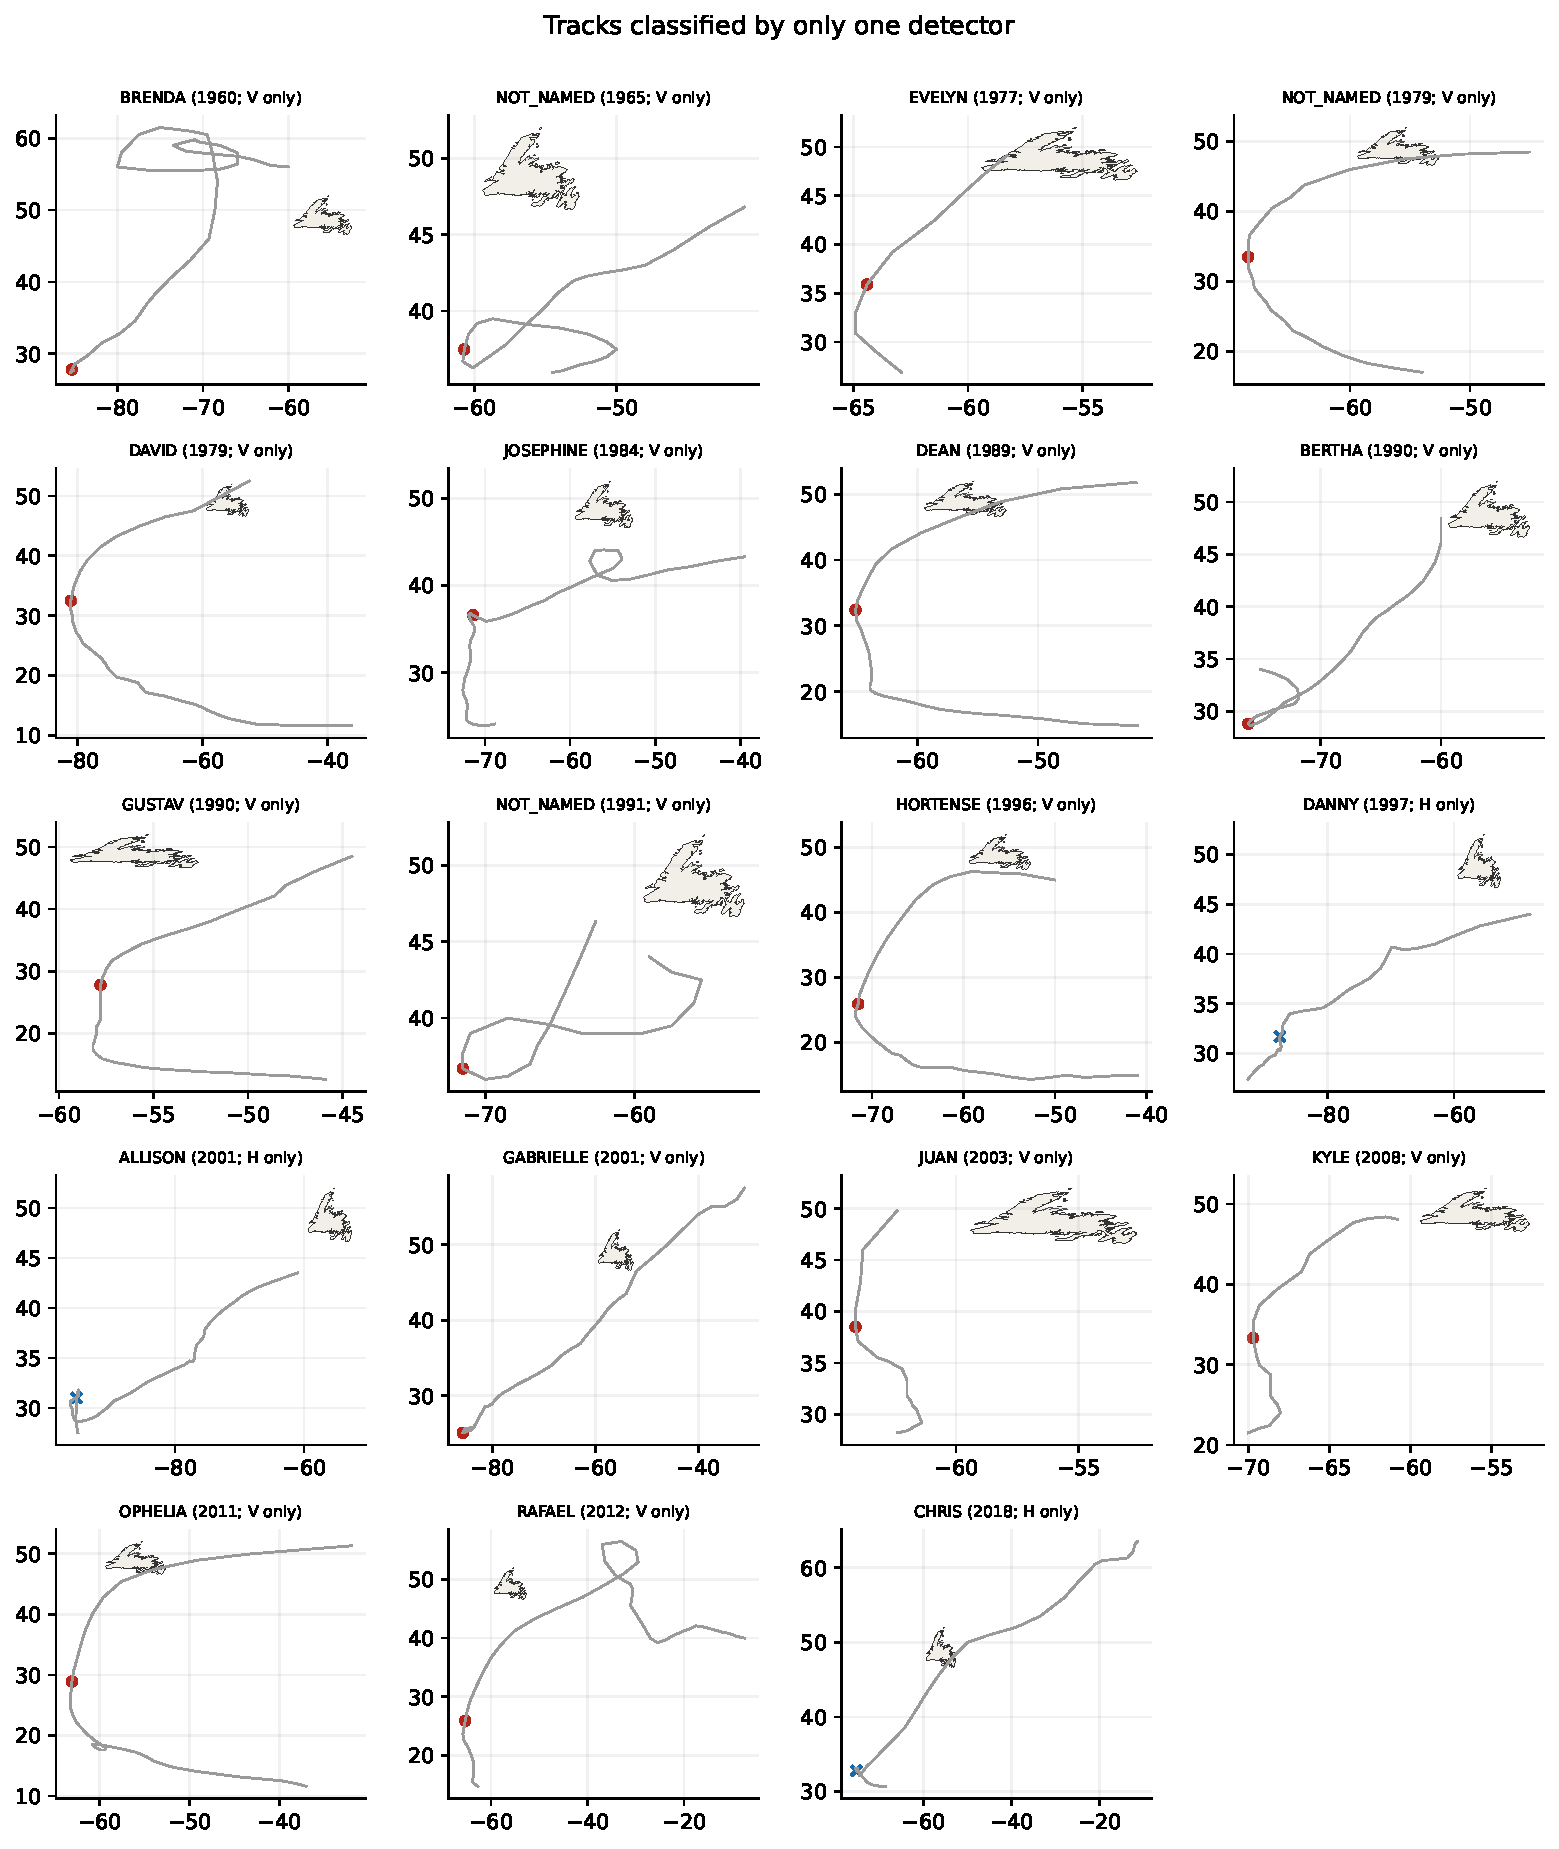
\includegraphics[width=0.90\textwidth]{figures/figA1_detector_discordant_tracks.pdf}
\caption{Tracks selected by only one of the baseline velocity and alternative heading detectors. Red circles mark velocity-detector recurvature points; blue crosses mark heading-detector points. ``V only'' and ``H only'' refer to the relevant-event lists after the same 600-km proximity screen.}
\label{fig:discordant}
\end{figure}

\section*{Data and code availability}
The executable notebook, source code, event lists, sensitivity tables, and generated composite fields accompany this manuscript. The public repository is \url{https://github.com/joeypeddle100/newfoundland-tc-recurvature}. A versioned release corresponding to this analysis should be archived before journal submission.

\begin{thebibliography}{9}

\bibitem[Knapp et~al.(2010)]{Knapp2010}
Knapp, K.~R., Kruk, M.~C., Levinson, D.~H., Diamond, H.~J., and Neumann, C.~J. (2010).
The International Best Track Archive for Climate Stewardship (IBTrACS): Unifying tropical cyclone best track data.
\textit{Bulletin of the American Meteorological Society}, \textit{91}, 363--376.
doi:10.1175/2009BAMS2755.1

\bibitem[Gahtan et~al.(2024)]{Gahtan2024}
Gahtan, J., Knapp, K.~R., Schreck, C.~J., Diamond, D.~H., Kossin, J.~P., and Kruk, M.~C. (2024).
International Best Track Archive for Climate Stewardship Project, Version 4.
NOAA National Centers for Environmental Information.
doi:10.25921/82ty-9e16

\bibitem[Kalnay et~al.(1996)]{Kalnay1996}
Kalnay, E., Kanamitsu, M., Kistler, R., Collins, W., Deaven, D., Gandin, L., Iredell, M., Saha, S., White, G., Woollen, J., Zhu, Y., and others (1996).
The NCEP/NCAR 40-Year Reanalysis Project.
\textit{Bulletin of the American Meteorological Society}, \textit{77}, 437--471.
doi:10.1175/1520-0477(1996)077<0437:TNYRP>2.0.CO;2

\bibitem[Landsea and Franklin(2013)]{LandseaFranklin2013}
Landsea, C.~W., and Franklin, J.~L. (2013).
Atlantic hurricane database uncertainty and presentation of a new database format.
\textit{Monthly Weather Review}, \textit{141}, 3576--3592.
doi:10.1175/MWR-D-12-00254.1

\bibitem[Evans and Hart(2003)]{EvansHart2003}
Evans, J.~L., and Hart, R.~E. (2003).
Objective indicators of the life cycle evolution of extratropical transition for Atlantic tropical cyclones.
\textit{Monthly Weather Review}, \textit{131}, 909--925.
doi:10.1175/1520-0493(2003)131<0909:OIOTLC>2.0.CO;2

\bibitem[Evans et~al.(2017)]{Evans2017}
Evans, C., Wood, K.~M., Aberson, S.~D., Archambault, H.~M., Milrad, S.~M., Bosart, L.~F., Corbosiero, K.~L., Davis, C.~A., and others (2017).
The extratropical transition of tropical cyclones. Part I: Cyclone evolution and direct impacts.
\textit{Monthly Weather Review}, \textit{145}(11), 4317--4344.
doi:10.1175/MWR-D-17-0027.1

\bibitem[Jones et~al.(2003)]{Jones2003}
Jones, S.~C., Harr, P.~A., Abraham, J., Bosart, L.~F., Bowyer, P.~J., Evans, J.~L., Hanley, D.~E., and others (2003).
The extratropical transition of tropical cyclones: Forecast challenges, current understanding, and future directions.
\textit{Weather and Forecasting}, \textit{18}(6), 1052--1092.
doi:10.1175/1520-0434(2003)018<1052:TETOTC>2.0.CO;2

\end{thebibliography}

\end{document}
